%  A simple AAU report template.
%  2015-05-08 v. 1.2.0
%  Copyright 2010-2015 by Jesper Kjær Nielsen <jkn@es.aau.dk>
%
%  This is free software: you can redistribute it and/or modify
%  it under the terms of the GNU General Public License as published by
%  the Free Software Foundation, either version 3 of the License, or
%  (at your option) any later version.
%
%  This is distributed in the hope that it will be useful,
%  but WITHOUT ANY WARRANTY; without even the implied warranty of
%  MERCHANTABILITY or FITNESS FOR A PARTICULAR PURPOSE.  See the
%  GNU General Public License for more details.
%
%  You can find the GNU General Public License at <http://www.gnu.org/licenses/>.
%
\documentclass[11pt,twoside,a4paper,openright]{report}
%%%%%%%%%%%%%%%%%%%%%%%%%%%%%%%%%%%%%%%%%%%%%%%%
% Language, Encoding and Fonts
% http://en.wikibooks.org/wiki/LaTeX/Internationalization
%%%%%%%%%%%%%%%%%%%%%%%%%%%%%%%%%%%%%%%%%%%%%%%%
% Select encoding of your inputs. Depends on
% your operating system and its default input
% encoding. Typically, you should use
%   Linux  : utf8 (most modern Linux distributions)
%            latin1 
%   Windows: ansinew
%            latin1 (works in most cases)
%   Mac    : applemac
% Notice that you can manually change the input
% encoding of your files by selecting "save as"
% an select the desired input encoding. 
\usepackage[utf8]{inputenc}
% Make latex understand and use the typographic
% rules of the language used in the document.
\usepackage[danish,english]{babel}
% Use the palatino font
\frenchspacing
\usepackage[sc]{mathpazo}
\linespread{1.05}         % Palatino needs more leading (space between lines)
% Choose the font encoding
\usepackage[T1]{fontenc}
%Symbol dictionary package(used for tick symbol)
\usepackage{bbding}

%%%%%%%%%%%%%%%%%%%%%%%%%%%%%%%%%%%%%%%%%%%%%%%%
% Graphics and Tables
% http://en.wikibooks.org/wiki/LaTeX/Importing_Graphics
% http://en.wikibooks.org/wiki/LaTeX/Tables
% http://en.wikibooks.org/wiki/LaTeX/Colors
%%%%%%%%%%%%%%%%%%%%%%%%%%%%%%%%%%%%%%%%%%%%%%%%
% load a colour package
\usepackage{xcolor}
\definecolor{aaublue}{RGB}{33,26,82}% dark blue
% The standard graphics inclusion package
\usepackage{graphicx}
% Set up how figure and table captions are displayed
\usepackage{subcaption}
\usepackage{caption}
\captionsetup{%
  font=footnotesize,% set font size to footnotesize
  labelfont=bf % bold label (e.g., Figure 3.2) font
}
% Make the standard latex tables look so much better
\usepackage{array,booktabs}
% Enable the use of frames around, e.g., theorems
% The framed package is used in the example environment
\usepackage{framed}

% Adds support for full page background picture
\usepackage[contents={},color=gray]{background}
%\usepackage[contents=draft,color=gray]{background}

%%%%%%%%%%%%%%%%%%%%%%%%%%%%%%%%%%%%%%%%%%%%%%%%
% Mathematics
% http://en.wikibooks.org/wiki/LaTeX/Mathematics
%%%%%%%%%%%%%%%%%%%%%%%%%%%%%%%%%%%%%%%%%%%%%%%%
% Defines new environments such as equation,
% align and split 
\usepackage{mathtools}
% Adds new math symbols
\usepackage{amssymb}
% Use theorems in your document
% The ntheorem package is also used for the example environment
% When using thmmarks, amsmath must be an option as well. Otherwise \eqref doesn't work anymore.
\usepackage[framed,amsmath,thmmarks]{ntheorem}

%%%%%%%%%%%%%%%%%%%%%%%%%%%%%%%%%%%%%%%%%%%%%%%%
% Page Layout
% http://en.wikibooks.org/wiki/LaTeX/Page_Layout
%%%%%%%%%%%%%%%%%%%%%%%%%%%%%%%%%%%%%%%%%%%%%%%%
% Change margins, papersize, etc of the document
\usepackage[
  inner=28mm,% left margin on an odd page
  outer=41mm,% right margin on an odd page
  headheight=13.6pt,
  bottom=39mm
  ]{geometry}
% Modify how \chapter, \section, etc. look
% The titlesec package is very configureable
\usepackage{titlesec}
\titleformat{\chapter}[display]{\normalfont\huge\bfseries}{\chaptertitlename\ \thechapter}{20pt}{\Huge}
\titleformat*{\section}{\normalfont\Large\bfseries}
\titleformat*{\subsection}{\normalfont\large\bfseries}
\titleformat*{\subsubsection}{\normalfont\normalsize\bfseries}
%\titleformat*{\paragraph}{\normalfont\normalsize\bfseries}
%\titleformat*{\subparagraph}{\normalfont\normalsize\bfseries}

% Clear empty pages between chapters
\let\origdoublepage\cleardoublepage
\newcommand{\clearemptydoublepage}{%
  \clearpage
  {\pagestyle{empty}\origdoublepage}%
}
\let\cleardoublepage\clearemptydoublepage

% Change the headers and footers
\usepackage{fancyhdr}
\pagestyle{fancy}
\fancyhf{} %delete everything
\renewcommand{\headrulewidth}{0pt} %remove the horizontal line in the header
\fancyhead[RE]{\small\nouppercase\leftmark} %even page - chapter title
\fancyhead[LO]{\small\nouppercase\rightmark} %uneven page - section title
\fancyhead[LE,RO]{\thepage \hspace{1pt} of \pageref{LastPage}} %page number on all pages
% Do not stretch the content of a page. Instead,
% insert white space at the bottom of the page
\raggedbottom
% Enable arithmetics with length. Useful when
% typesetting the layout.
\usepackage{calc}

%%%%%%%%%%%%%%%%%%%%%%%%%%%%%%%%%%%%%%%%%%%%%%%%
% Bibliography
% http://en.wikibooks.org/wiki/LaTeX/Bibliography_Management
%%%%%%%%%%%%%%%%%%%%%%%%%%%%%%%%%%%%%%%%%%%%%%%%
\usepackage[backend=biber,
  bibencoding=utf8,
  maxbibnames=20,
  style=numeric-comp,
  sorting=none
  ]{biblatex}
\addbibresource{bib/mybib.bib}
\usepackage{microtype} %Prevent overfull issues in bibliography

%%%%%%%%%%%%%%%%%%%%%%%%%%%%%%%%%%%%%%%%%%%%%%%%
% Misc
%%%%%%%%%%%%%%%%%%%%%%%%%%%%%%%%%%%%%%%%%%%%%%%%
% Add bibliography and index to the table of
% contents
\usepackage[nottoc]{tocbibind}
% Add the command \pageref{LastPage} which refers to the
% page number of the last page
\usepackage{lastpage}
% Add todo notes in the margin of the document
\usepackage[
%  disable, %turn off todonotes
  colorinlistoftodos, %enable a coloured square in the list of todos
  textwidth=\marginparwidth, %set the width of the todonotes
  textsize=scriptsize, %size of the text in the todonotes
  ]{todonotes}

%%%%%%%%%%%%%%%%%%%%%%%%%%%%%%%%%%%%%%%%%%%%%%%%
% Code listings and pseudocode
\usepackage[newfloat]{minted}
\setminted[python]{frame=topline, framesep=6pt, style=colorful, fontsize=\footnotesize, linenos, breaklines, autogobble} %Change language later
\setminted[c]{frame=topline, framesep=6pt, style=colorful, fontsize=\footnotesize, linenos, breaklines, autogobble}
\setminted[antlr]{frame=topline, framesep=6pt, fontsize=\footnotesize, linenos, breaklines, autogobble}

\setminted[arduino]{frame=topline, framesep=6pt, fontsize=\footnotesize, linenos, breaklines, autogobble}


\usepackage{clrscode3e}
\DeclareFloatingEnvironment[name=Algorithm, placement=htpb]{algorithm} %Create Algorithm float
%%%%%%%%%%%%%%%%%%%%%%%%%%%%%%%%%%%%%%%%%%%%%%%%
% Hyperlinks
% http://en.wikibooks.org/wiki/LaTeX/Hyperlinks
%%%%%%%%%%%%%%%%%%%%%%%%%%%%%%%%%%%%%%%%%%%%%%%%
% Enable hyperlinks and insert info into the pdf
% file. Hypperref should be loaded as one of the 
% last packages
\usepackage[hidelinks]{hyperref}
\hypersetup{%
	plainpages=false,%
	pdfauthor={Author(s)},%
	pdftitle={Title},%
	pdfsubject={Subject},%
	bookmarksnumbered=true,%
	colorlinks=false,%
	citecolor=black,%
	filecolor=black,%
	linkcolor=black,% you should probably change this to black before printing
	urlcolor=black,%
	pdfstartview=FitH%
}
\usepackage{tabularx} % tabel formattering
\usepackage{booktabs} % tabel formattering
\usepackage{multirow} % multiple columns and rows

\usepackage{listings}

\usepackage[autostyle, threshold=0]{csquotes}% package inclusion and set up of the document
% see, e.g., http://en.wikibooks.org/wiki/LaTeX/Formatting#Hyphenation
% for more information on word hyphenation
\hyphenation{ex-am-ple hy-phen-a-tion short}
\hyphenation{long la-tex}
% 
\newcommand{\aautitlepage}[3]{%
  {
    %set up various length
    \ifx\titlepageleftcolumnwidth\undefined
      \newlength{\titlepageleftcolumnwidth}
      \newlength{\titlepagerightcolumnwidth}
    \fi
    \setlength{\titlepageleftcolumnwidth}{0.5\textwidth-\tabcolsep}
    \setlength{\titlepagerightcolumnwidth}{\textwidth-2\tabcolsep-\titlepageleftcolumnwidth}
    %create title page
    \thispagestyle{empty}
    \noindent%
    \begin{tabular}{@{}ll@{}}
      \parbox{\titlepageleftcolumnwidth}{
        \iflanguage{danish}{%
          
\includegraphics[width=\titlepageleftcolumnwidth]{AAUgraphics/aau_logo_da}
        }{%
          
\includegraphics[width=\titlepageleftcolumnwidth]{AAUgraphics/aau_logo_en}
        }
      } &
      \parbox{\titlepagerightcolumnwidth}{\raggedleft\sf\small
        #2
      }\bigskip\\
       #1 &
      \parbox[t]{\titlepagerightcolumnwidth}{%
      \textbf{Abstract:}\par
        \fbox{\parbox{\titlepagerightcolumnwidth-2\fboxsep-2\fboxrule}{%
          #3
        }}
      }\\
    \end{tabular}
    \vfill
    \iflanguage{danish}{%
      \noindent{\footnotesize\emph{Rapportens indhold er frit tilgængeligt, men offentliggørelse (med kildeangivelse) må kun ske efter aftale med forfatterne.}}
    }{%
      \noindent{\footnotesize\emph{The content of this report is freely available, but publication (with reference) may only be pursued due to agreement with the author.}}
    }
    \clearpage
  }
}

%Create english project info
\newcommand{\englishprojectinfo}[8]{%
  \parbox[t]{\titlepageleftcolumnwidth}{
    \textbf{Title:}\\ #1\bigskip\par
    \textbf{Theme:}\\ #2\bigskip\par
    \textbf{Project Period:}\\ #3\bigskip\par
    \textbf{Project Group:}\\ #4\bigskip\par
    \textbf{Participant(s):}\\ #5\bigskip\par
    \textbf{Supervisor(s):}\\ #6\bigskip\par
    \textbf{Copies:} #7\bigskip\par
    \textbf{Page Numbers:} \pageref{LastPage}\bigskip\par
    \textbf{Date of Completion:}\\ #8
  }
}

%Create danish project info
\newcommand{\danishprojectinfo}[8]{%
  \parbox[t]{\titlepageleftcolumnwidth}{
    \textbf{Titel:}\\ #1\bigskip\par
    \textbf{Tema:}\\ #2\bigskip\par
    \textbf{Projektperiode:}\\ #3\bigskip\par
    \textbf{Projektgruppe:}\\ #4\bigskip\par
    \textbf{Deltager(e):}\\ #5\bigskip\par
    \textbf{Vejleder(e):}\\ #6\bigskip\par
    \textbf{Oplagstal:} #7\bigskip\par
    \textbf{Sidetal:} \pageref{LastPage}\bigskip\par
    \textbf{Afleveringsdato:}\\ #8
  }
}

%%%%%%%%%%%%%%%%%%%%%%%%%%%%%%%%%%%%%%%%%%%%%%%%
% An example environment
%%%%%%%%%%%%%%%%%%%%%%%%%%%%%%%%%%%%%%%%%%%%%%%%
\theoremheaderfont{\normalfont\bfseries}
\theorembodyfont{\normalfont}
\theoremstyle{break}
\def\theoremframecommand{{\color{gray!50}\vrule width 5pt \hspace{5pt}}}
\newshadedtheorem{exa}{Example}[chapter]
\newenvironment{example}[1]{%
		\begin{exa}[#1]
}{%
		\end{exa}
}

%%%%%%%%%%%%%%%%%%%%%%%%%%%%%%%%%%%%%%%%%%%%%%%%
% Specialized todo macros
%%%%%%%%%%%%%%%%%%%%%%%%%%%%%%%%%%%%%%%%%%%%%%%%
\newcommand{\supervisor}[2][]{\todo[color=green!50,#1]{#2}}
\newcommand{\question}[2][]{\todo[color=cyan!30,#1]{#2}}
\newcommand{\urgent}[2][]{\todo[color=red!50,#1]{#2}}
\newcommand{\feedback}[2][]{\todo[color=teal!70,#1]{#2}}% my new macros

\makeglossaries% import glossaries
\loadglsentries{setup/acronyms.tex}

\begin{document}
%frontmatter
\pagestyle{empty} %disable headers and footers
\pagenumbering{roman} %use roman page numbering in the frontmatter
\pdfbookmark[0]{Front page}{label:frontpage}%
\begin{titlepage}
\vspace*{\fill}
    \backgroundsetup{
    scale=1.1,
    angle=0,
    opacity=1.0,  %% adjust
    contents={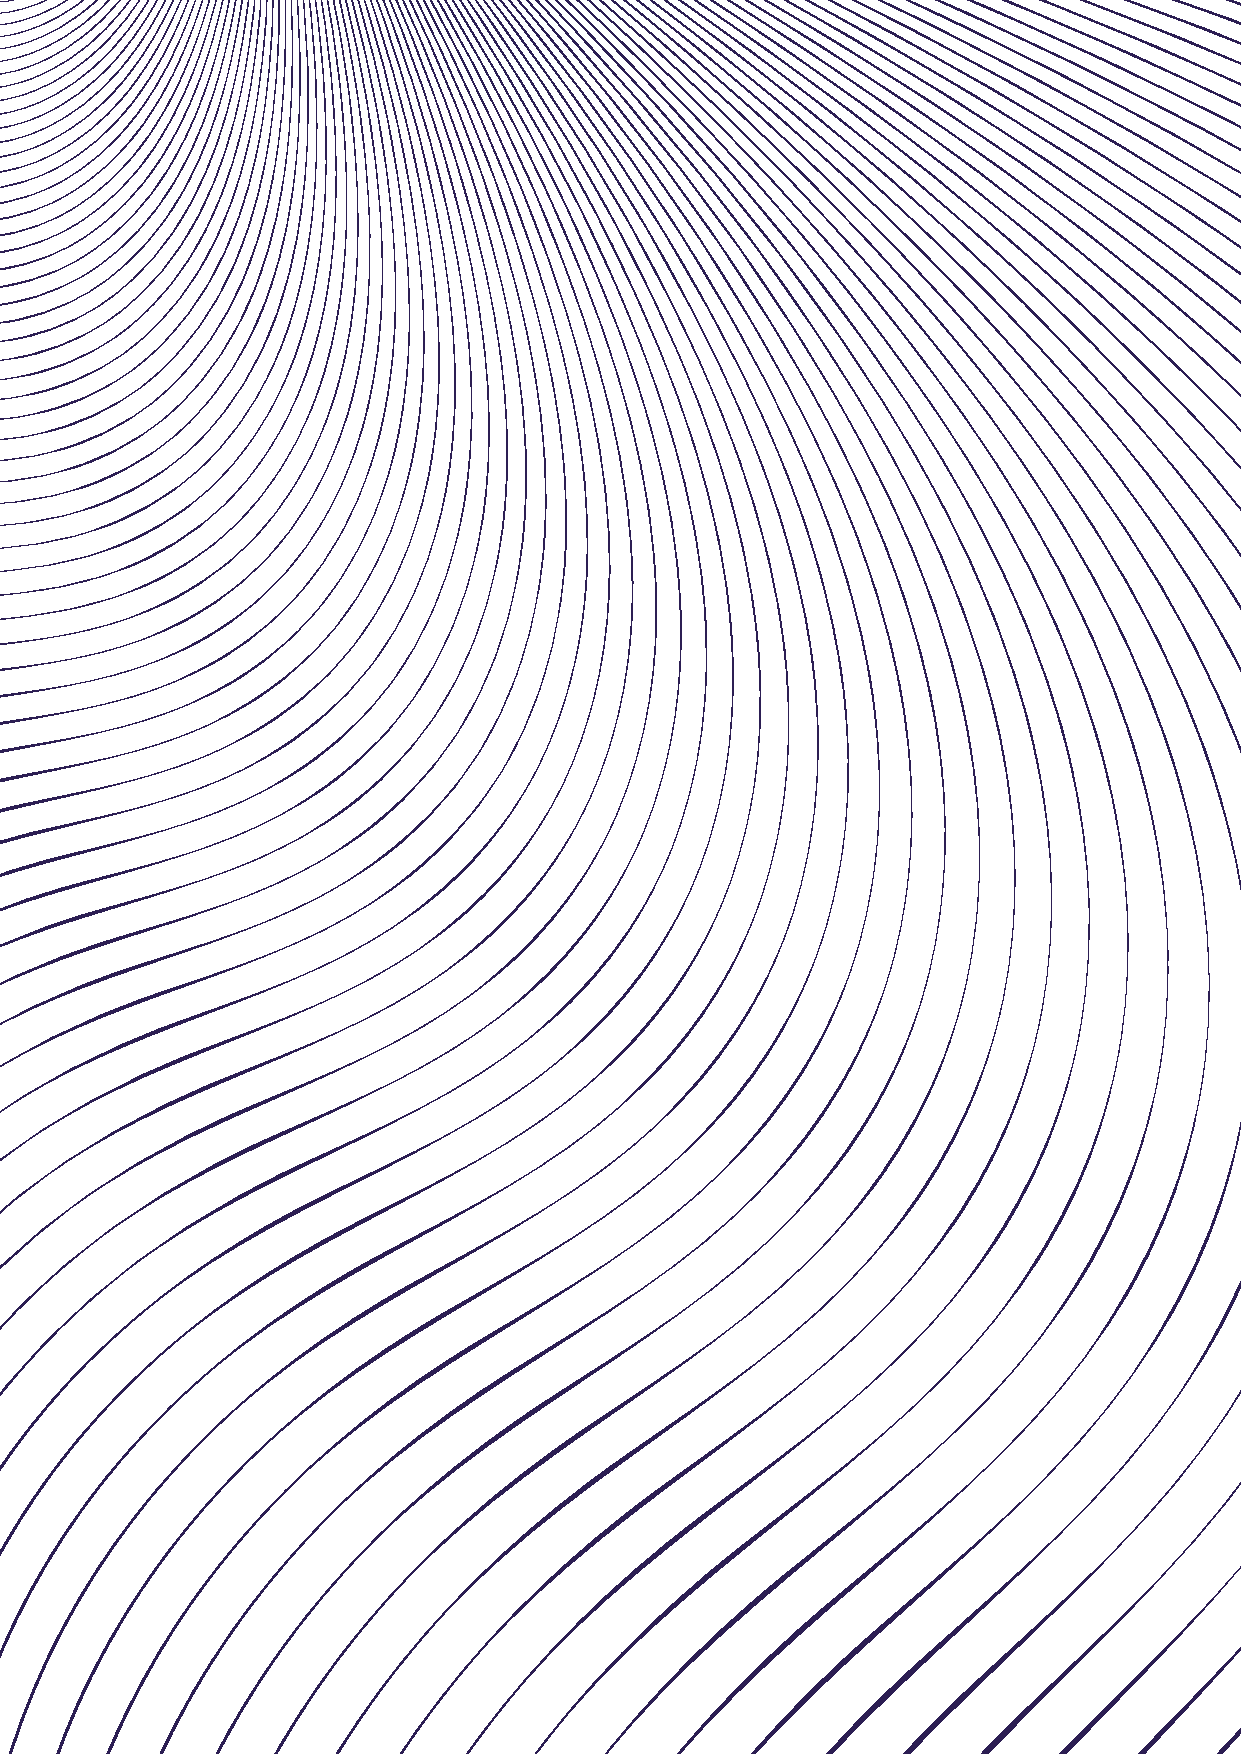
\includegraphics[width=\paperwidth,height=\paperheight]{AAUgraphics/aau_waves}}
    }
  \addtolength{\hoffset}{0.5\evensidemargin-0.5\oddsidemargin} %set equal margins on the frontpage - remove this line if you want default margins
  \noindent%
  {\color{white}\fboxsep0pt\colorbox{aaublue}{\begin{tabular}{@{}p{\textwidth}@{}}
    \begin{center}
    \Huge{\textbf{
      Concurrency in Arduino% insert your title here
    }}
    \end{center}
    \begin{center}
      \Large{
        Development of the Arc programming language% insert your subtitle here
      }
    \end{center}
    \vspace{0.2cm}
   \begin{center}
    {\Large
      Christoffer Trebbien Jønsson, Daniel Runge Petersen, Gustav Svante Grønkjær Graversen, Jamie Lee Smith Hammer, Lars Emanuel Hansen, Sebastian Aaholm% insert names separated by comma
    }\\
    \vspace{0.2cm}
    {\large
      Computer Science, cs-22-dat-4-03, 2022-05% insert name of study, group number, year-month
    }
   \end{center}
   \vspace{0.2cm}
%% Comment this section in if you are doing Bachelor or Master Project   
   \begin{center}
    {\Large
      Semester Project
      %Bachelor Project
    }
   \end{center}
  \end{tabular}}}
  \vfill
  \begin{center}
    
\includegraphics[width=0.2\paperwidth]{AAUgraphics/aau_logo_circle_en}% comment this line in for English version
    %
\includegraphics[width=0.2\paperwidth]{AAUgraphics/aau_logo_circle_da} %comment this line in for Danish version
  \end{center}
\end{titlepage}
\clearpage

\thispagestyle{empty}
{\small
\strut\vfill % push the content to the bottom of the page
\noindent Copyright \copyright{} Aalborg University 2021\par
\vspace{0.2cm}
\noindent Here you can write something about which tools and software you have used for typesetting the document, running simulations and creating figures. If you do not know what to write, either leave this page blank or have a look at the colophon in some of your books.
}
\clearpage


\pdfbookmark[0]{English title page}{label:titlepage_en}
\aautitlepage{%
  \englishprojectinfo{
    Concurrency in Arduino %title
  }{%
    Design definition and implementation programming languages %theme
  }{%
    Spring Semester 2022 %project period
  }{%
    cs-22-dat-4-03 % project group
  }{%
    %list of group members
    Christoffer Trebbien Jønsson\\ 
    Daniel Runge Petersen\\
    Gustav Svante Grønkjær Graversen\\
    Jamie Lee Smith Hammer\\
    Lars Emanuel Hansen\\
    Sebastian Aaholm
  }{%
    %list of supervisors
    Giovanni Bacci
  }{%
    1 % number of printed copies
  }{%
    \today % date of completion
  }%
}{%department and address
  \textbf{Electronics and IT}\\
  Aalborg University\\
  \href{http://www.aau.dk}{http://www.aau.dk}
}{% the abstract
  Here is the abstract
}



\cleardoublepage


\pdfbookmark[0]{Contents}{label:contents}
\pagestyle{fancy} %enable headers and footers again
\setcounter{tocdepth}{1} %determine depth of table of contents. 0 - 4
\tableofcontents

\todototoc\listoftodos

\chapter*{Preface\markboth{Preface}{Preface}}\label{ch:preface}
\addcontentsline{toc}{chapter}{Preface}
Here is the preface. You should put your signatures at the end of the preface.

\vspace{\baselineskip}\hfill Aalborg University, \today
\vfill\noindent
\begin{minipage}[b]{0.45\textwidth}
 \centering
 \rule{\textwidth}{0.5pt}\\
  Author 1\\
 {\footnotesize <username1@XX.aau.dk>}
\end{minipage}
\hfill
\begin{minipage}[b]{0.45\textwidth}
 \centering
 \rule{\textwidth}{0.5pt}\\
  Author 2\\
 {\footnotesize <username2@XX.aau.dk>}
\end{minipage}
\vspace{3\baselineskip}
\begin{center}
\begin{minipage}[b]{0.45\textwidth}
 \centering
 \rule{\textwidth}{0.5pt}
  Author 3\\
 {\footnotesize <username3@XX.aau.dk>}
\end{minipage}
\end{center}

\cleardoublepage


%mainmatter
\pagenumbering{arabic} %use arabic page numbering in the mainmatter

\chapter{Introduction}\label{cha:introduction}
This report details the design, definition, and implementation of a programming language, as per \gls{aau}'s fourth-semester module description \cite{AAU_Modules_P4}. The programming language is named Arco for \textit{Arduino Concurrently}, and its purpose is to make is a little simpler to write concurrent programs for the arduino.

\section{Initial problem}\label{sec:initialproblem}
The problem analysis begins from the project proposal: "A Concurrent Programming Language for Arduino". The proposal outlines how microcontrollers, like the Arduino, are used in \gls{cps} to monitor and control the surroundings. However, although sensor input is sent asynchronously with regards to the \gls{cpu} the Arduino has no direct support for concurrency.

\subsection{Project outline}
The project proposal presents the following tasks and challenges:

\paragraph{Tasks}
\begin{itemize}
    \item Develop a language that integrates Concurrent tasks in Arduino
    \item Give natural support to the \gls{cps} feedback loop
    \item It should have an intuitive domain specific syntax
\end{itemize}

\paragraph{Challenges}
\begin{itemize}
    \item Handle context switch taking \textbf{real-time constraints} in mind
    \item Provide constructs to handle \textbf{race conditions} (atomic sessions, semaphores, asynchronous queues, etc.)
    \item Comply with memory requirements
\end{itemize}


\chapter{Problem analysis}\label{cha:problemanalysis}
This chapter details the problem analysis, from the initial problem to a problem statement. Based on the initial problem, a set of questions to research during the problem analysis has been determined:

\begin{description}
    \item[Arduino] What is Arduino, and who uses it? What is the Arduino programming language?
    \item[Concurrency] What is concurrency, and what does it mean to work concurrently? What are the different approaches/models for concurrency, and what are the challenges in relation to Arduino?
\end{description}

\section{Arduino}\label{sec:arduino}
Arduino is an open-source electronics platform that enables users to quickly create small microcontroller projects through easy-to-use hardware and software \cite{WhatArduino}. Multiple variants of Arduino boards exist, with different components and specifications. The UNO, Due, Mega2560, Micro, Leonardo, Zero, Mini, and UNO WiFi are within the classic family of Arduino boards. Because of Arduino being an open-source project, other companies are free to use the specifications to provide third-party implementations of the boards.

\todo{Kig på første sætning}
An Arduino UNO is used as the reference board for this project because \gls{aau} has provided one. All physical tests and examples will run on this board, and the implementation will depend on the Arduino UNO specification henceforth.

The software for the Arduino is the official Arduino IDE, in which developers can write code in the Arduino programming language. The IDE and the programming language is built on Wiring, which builds on Processing \cite{WhatArduino,WiringOrg}.

\subsection{The Arduino programming language}\label{subsec:arduinoprogramminglanguage}
The Arduino programming language closely resembles the C programming language and is, in fact, a set of C/C++ functions \cite{ArduinoSupportC}. It contains most of the constructs of C++, with some additional functions added and a few features, turned off in the compiler, such as exceptions \cite{Nongnuorg}.

\subsubsection{Sketches}
A program written in the Arduino IDE and programming language is called a sketch. A sketch follows a basic structure that consists of implementing the procedures "setup()" and "loop()". Setup is a procedure called once during a run - when the Arduino is turned on or reset; it initializes variables, pin modes, libraries, and some additional links. After setup, the loop begins. The loop procedure is a loop that runs for the duration of the runtime of the program and contains the logic of the project \cite{ArduinoLanguage}.

\subsection{Who uses the Arduino?}\label{subsec:whouses}
A wide range of people, such as students, hobbyists, children, programmers, and professionals, use Arduino for many different purposes \cite{WhatArduino}. Some are focused on the learning aspects of the Arduino - architecture, code, and embedded systems, while others are more interested in designing product concepts. Students and children can use the board to learn the basics of electronics; hobbyists may use it to build personal \gls{diy} projects, while professionals often use it to design product concepts \cite{WhatArduino}.

Designing a programming language for dedicated programmers or professionals may require a profound understanding of many underlying details of the Arduino platform itself. Providing a good language for these groups can potentially detract from the project's purpose - which is to design a programming language - because it may take more time than is available to obtain this knowledge. Thus, this is not the target group. The project also will not deal with a programming language designed for children, as this would require an understanding of pedagogical tools, which is outside the scope of a computer science education.

The hobbyist is, however, an excellent group for which to design our implementation for. Because hobbyists spend their leisure time on Arduino projects, the primary concerns are their limited available time and the potential for frustration during a project. Moreover, hobbyists might have limited programming proficiency or be complete beginners. The standard Arduino language already alleviates many problems, but not in regards to concurrency. The user group for the remainder of this report is hobbyists who want to do as much as they can with their limited time and limited coding proficiency - specifically related to concurrency.
\section{Concurrency}\label{sec:concurrency}
The term concurrency is a general term for ways a computer system performs multiple tasks simultaneously. It covers the \textit{simulation} of multiple tasks running at the same time through process switching, as well as work done in parallel. To disambiguate, based on the definition:

\blockcquote{Bryant2016}{We use the term concurrency to refer to the general concept of a system with multiple, simultaneous activities, and the term parallelism to refer to the use of concurrency to make a system run faster.}

We infer that parallelism is a type of concurrency to speed up the system, while concurrency, in general, may have purposes not related to speed, for example, synchronization of tasks.

Concurrency is a complex, large, and hardware-dependent subject~\cite{Sebesta2016}. The limitations of the Arduino hardware concerning concurrency, specifically the \gls{cpu}, are explored before concurrency in general because the project is, first and foremost, about programming language design - not concurrency.

\subsection{Arduino hardware}\label{subsec:arduinohardware}
The Arduino Uno board uses the ATmega328P microcontroller~\cite{ArduinoUno}. The architecture of this microcontroller is a scalar single-core processor without hyperthreading(intel) or \gls{smt} (AMD) equivalents~\cite{ATmega328P}.

Since there only exists a single core, which does not contain any duplicate copies of CPU hardware (for multithreading), the only hardware parallelism on the Arduino Uno is instruction-level parallelism, and only to the level of up to 1 instruction per clock cycle (scalar). This parallelism is also handled directly by the \gls{cpu} and does not impact the instruction set available to developers.


\begin{figure}[htb!]
    \centering
    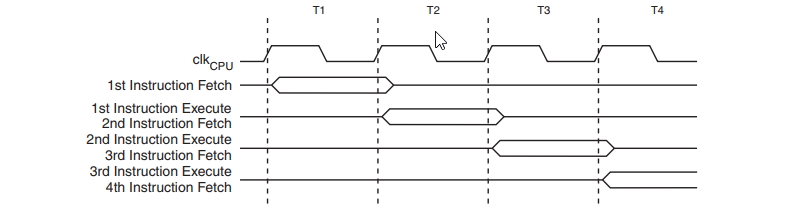
\includegraphics[width=\textwidth]{figures/Arduino_Pipeline.png}
    \caption{The parallel intruction fetches and intruction executions \cite{ATmega328P}}
    \label{fig:arduinopipeline}
\end{figure}


Therefore, the Arduino is a uniprocessor~\cite{Bryant2016} whose architecture does not support parallel processing - and for the remainder of the report, the term concurrency refers to concurrency \textbf{without parallelism}.

Even unicore processors can support several models for concurrency at the application software level, which makes sense since most computers often have more processes running than \glspl{cpu}. Achieving this concurrency is done through interleaving instructions of different processes, which lets the \gls{cpu} appear to run multiple programs.

This interleaving is commonly handled by an \gls{os}, which manages the hardware resources~\cite{Bryant2016}. However, by default, the Arduino does not have an \gls{os}. It is still possible to achieve concurrency on an Arduino, but not without a scheduler or scheduling.

\subsection{Concurrency on an Arduino}\label{subsec:concurrencyinarduino}
The scheduler is the part of the \gls{os} that handles the planning and switching of different tasks on the CPU within the system. However, an \gls{os} is not the only way to obtain scheduling behavior. Several online tutorials~\cite{BadExample1, BadExample2} demonstrate different techniques to achieve concurrency on an Arduino, such as using the Arduino functions millis() and interrupt().

The millis() technique executes different pieces of code depending on some programmer-defined timeslices and comparisons between the current time and an earlier time. The interrupt() method uses the \gls{cpu} interrupt command to interrupt the \gls{cpu} and restart it from another place in the code.

Both methods require the programmer to think deeply about how they wish for the program to execute, which can get complicated and frustrating fast. The interrupt() case is a very low-level command that might not work entirely as a novice or hobbyist expects. In the case of the millis() method, it requires many global variables to execute the program correctly, which can be difficult. In both cases, the code may be hard to maintain or understand.

These examples highlight a general difficulty with the Arduino model, and several solutions to the described problems exist, some of which are explored in the next section.

\section{Existing solutions}\label{sec:existingsolutions}
In this section, some ways of achieving concurrency on an Arduino is explored. Emphasis is put on the immediate advantages and disadvantages related to each model, when considering the impact on the hobbyist users, by which is meant the new challenges, if any, introduced by the model in question.

A small sample project is implemented in each model for the sake of comparison: The builtin \gls{led} of the Arduino is set to blink - turn on and off - every half second. Concurrently, the state of a button is read and printed continously. The example will be implemented in the Arc programming language as well. The schematic for the project is seen in Figure ~\ref{fig:exampleprojectschematic}.


\begin{figure}[htb!]
  \centering
  \missingfigure[figwidth=0.8\textwidth]{Insert image of Arduino schematic?}
  %\includegraphics[width=0.8\textwidth]{example-image-a}
  \caption{Example project schematic}
  \label{fig:exampleprojectschematic}
\end{figure}


The first discussion is about the prospect of using programming libraries to achieve concurrency on an Arduino. The second discussion is about the possibility of installing an \gls{os} on the Arduino, and building on the \gls{os}-exposed concurrency abstractions.

\subsection{Concurrency through Arduino libraries}\label{subsec:arduinolibraries}
In this section, the \textit{Protothreads} and \textit{Eventually} libraries are explored and compared. Of particular concern is the quality of the documentation, the model of concurrency, and the overhead of usage on the Arduino.

\subsubsection{Protothreads}
Protothreads is a library for the C language, which has been implemented as a library for Arduino \cite{Artin2020}. It is based on Adam Dunkels protothreads ~\cite{AdamDunkelProtothreads}.


\blockcquote{Artin2020, AdamDunkelProtothreads}{Protothreads provides a blocking context on top of an event-driven system, without the overhead of per-thread stacks. The purpose of protothreads is to implement sequential flow of control without complex state machines or full multi-threading.}


\begin{listing}[htb!]
  \centering
  \begin{minted}[label=Protothreads example]{arduino}
    #include "protothreads.h"
    const int buttonPin = 12; const int ledPin = 8;
    int buttonState = 0;  // variable for reading the pushbutton status
    pt ptBlink, ptButton;

    int blinkThread(struct pt *pt) {
      PT_BEGIN(pt);
      for (;;) {
        digitalWrite(ledPin, HIGH); // turn the LED on (HIGH is the voltage level)
        PT_SLEEP(pt, 500);
        digitalWrite(ledPin, LOW); // turn the LED off by making the voltage LOW
        PT_SLEEP(pt, 500);
      }
      PT_END(pt);
    }

    int buttonThread(struct pt *pt) {
      PT_BEGIN(pt);
      for (;;) {
        buttonState = digitalRead(buttonPin);
        Serial.println(buttonState);
        PT_YIELD(pt);
      }
      PT_END(pt);
    }

    void setup() {
      PT_INIT(&ptBlink);
      PT_INIT(&ptButton);
      Serial.begin(9600);
      pinMode(ledPin, OUTPUT);
      pinMode(buttonPin, INPUT);
    }

    void loop() {
      PT_SCHEDULE(blinkThread(&ptBlink));
      PT_SCHEDULE(buttonThread(&ptButton));
    }
  \end{minted}
  \caption{A small example on how a Protothreads can be implemented}
  \label{lst:protothreadsexample}
\end{listing}


The pitch for Protothreads is promising, and directly addresses the concern about overhead. However it does not describe the model of concurrency in great detail. Fortunately the documentation is excellent on both the Arduino implementation ~\cite{Artin2020} as well as the general Protothreads specification ~\cite{AdamDunkelProtothreads}.

Protothreads uses a cooperative form of concurrency, which means it is us tp the user to synchronize the program. This means that a program written with protothreads is event-driven and blocking - it must finish, or pause, explicitly, before moving on to the next task.

Protothreads is also implemented on a single stack with stack rewinding, unlike traditional multithreadings which has a stack per thread. This is the reason for the low overhead of Protothreads. On the Arduino, this is achieved through utilization of \textbf{local continuations} - threads are simply a struct with an unsigned short - together with macros that expand to a switch statement with a number of returns. The short contained in the thread is the set and compared against the switch defined by the macros to set the state and continuation.

Because threads are a struct with a short, they have a size of only two bytes. This means that there is no hidden memory cost during the execution of the program. However, the implementation details of the Protothread library does have a few effects on how to write programs when using it. 

First, a protothread only saves the short across blocking calls. This means that local variables inside a thread are not preserved - a rule of thumb from the designer is that local variables simply should not be used inside a protothread. Instead, it is prudent to use global variables, if data should be preserved.

% BEGIN HERE FRIDAY
Secondly, the scheduling of protothreads uses a switch statement in a way that prevents 




Lastly, it is important that the code inside a Protothread needs to be "fast", meaning that the programmer should not use any of the arduino cpu blocking functions, such as the delay() function, because this would block the other functions to run. ~\cite{AdamDunkelProtothreads}

The implementation of our sample project with protothreads can be seen in Listing ~\ref{lst:protothreadsexample}.






%---Links to Eventually c++ Libary---
%1. https://github.com/johnnyb/Eventually
%2. https://www.arduino.cc/reference/en/libraries/eventually/
% What is Eventually C++ Library?
% Advantages and disadvantages of Eventually Library (C++ issues)

\subsubsection{Eventually}
% From what I have found there is basic two valid sources which shortly explain what the Eventually C++ Library is and then there is some smaller code examples that show how to use it. So i don't know how relevant it is to have in the report since is just an other way of making event-bases programming like protothreads?
Eventually is an Arduino Event-based Programming Library. Where the goal is to make a more event-oriented environment for the Arduino programming language.

To give a better understanding of how the Eventually C++ library is working, in this section there has been taken an example from a GitHub page ~\cite{bartlettEventually2022Bartlett} where there can be seen, a code example on how to use the Eventually library. Since it is a C++ library it would work on any Arduino board, which includes the one the group has acquired.


\begin{listing}
  \begin{minted}[label=Eventually example]{arduino}
    #include <Eventually.h>
    #define LIGHT_PIN 8
    #define BUTTON_PIN 12
    bool pinState = true;
    EvtManager mgr;

    bool blinker() {
      mgr.resetContext();
      mgr.addListener(new EvtTimeListener(1000, true, (EvtAction)blink_pin)); 
      mgr.addListener(new EvtPinListener(BUTTON_PIN, (EvtAction)digital_read));
    }

    void blink_pin() {
      if (pinState == true) {
        digitalWrite(LIGHT_PIN, HIGH);
      } else {
        digitalWrite(LIGHT_PIN, LOW);
      }
      pinState = !pinState;
    }

    void digital_read() {
        int sensorVal = digitalRead(BUTTON_PIN);
        Serial.println(sensorVal);
        delay(1);
    }

    void setup() {
      Serial.begin(9600);
      pinMode(LIGHT_PIN, OUTPUT);
      pinMode(BUTTON_PIN, INPUT);
      blinker();
    }

    USE_EVENTUALLY_LOOP(mgr)
  \end{minted}
  \caption{A small program on how Eventually can be implemented}
  \label{lst:eventuallyexample}
\end{listing}


\subsection{Achieving Concurrency with an Operating System}



%---Links to Free rtos---
%1. https://github.com/feilipu/Arduino_FreeRTOS_Library
%   Forklar hvad link går ud på
\subsubsection{FreeRTOS}
Free Real-Time Operating System (abbreviated to FreeRTOS) is an operating system specifically designed for microcontrollers and microcomputers, such as the Arduino. It has been developed in partnership with the leading chip companies in the world, over more than 18 years, and with a special emphasis on reliability, accessibility and ease of use ~\cite{AboutRTOS}. This leads itself well to our project, while we are targeting hobbyists. FreeRTOS utilises preemptive scheduling ~\cite{SchedulingRTOS}, which means that it implements a scheduler to be responsible for deciding which tasks to do in which order.



\begin{listing}[htb!]
  \centering
  \begin{minted}[label=FreeRTOS example]{arduino}
#include <Arduino_FreeRTOS.h>

void TaskBlink(void *pvParameters){ // This is a task.
  (void) pvParameters;
  pinMode(LED_BUILTIN, OUTPUT);
  for (;;) { // A Task shall never return or exit.
    digitalWrite(LED_BUILTIN, HIGH);
    vTaskDelay( 1000 / portTICK_PERIOD_MS );
    digitalWrite(LED_BUILTIN, LOW);
    vTaskDelay( 1000 / portTICK_PERIOD_MS );
  }
}

void TaskAnalogRead(void *pvParameters){ // This is a task.
  (void) pvParameters;
  for (;;) {
    int sensorValue = digitalRead(12);
    Serial.println(sensorValue);
    vTaskDelay(1);
  }
}

void setup() {
  Serial.begin(9600);
  while (!Serial) {;}
  xTaskCreate(TaskBlink, "Blink", 128, NULL, 2, NULL);
  xTaskCreate(TaskAnalogRead, "AnalogRead", 128, NULL, 1, NULL);
}

void loop(){}
\end{minted}
  \caption{A small example of a possible implementation of Free RTOS.}
  \label{lst:freeftosexample}
\end{listing}

%and Preemptive concurrency forms \cite{UsingFreeRTOSMultitasking}, the preemptive concurrency form is priority-based, like the cooperative concurrency form the preemptive concurrency form has to prioritise the tasks in the program, but a task has to be completed in the time period which the scheduler has given task, it then switches to another task and if the first task was not completed it switches back \cite{Windows}.
%the library has a scheduler to set up when the tasks have to be executed, the programmer can also set up when the Arduino has to do a specific task, if no specific timed workflow, the scheduler assigns the priority of the tasks \cite{UsingFreeRTOSMultitasking}. 

%---Links to Simba library---
% 1. https://simba-os.readthedocs.io/en/latest/
%   Forklar hvad link går ud på
% 2. https://all3dp.com/2/best-arduino-operating-system/
%   Forklar hvad link går ud på
%\subsubsection{Simba}



%---Links to TaskManagerIO library---
% 1. https://github.com/davetcc/TaskManagerIO
%   Forklar hvad link går ud på
% 2. https://all3dp.com/2/best-arduino-operating-system/
%   Forklar hvad link går ud på
%\subsubsection{TaskManagerIO }




It is also possible to install an \gls{os} on the Arduino, and obtain a scheduler (and other things) that way.

\subsection*{Deprecated at the moment}
\subsection{Models of concurrency}\label{subsec:modelsofcon}
% might be relevant to explain the concurrency models of an OS, to compare the choices.
This interleaving is commonly handled through an \gls{os}, which manages the hardware resources ~\cite{Bryant2016}. A few different approaches for interleaving processes are supported by most \glspl{os}:

\subsubsection{Processes}
In this model the kernel, the portion of the \gls{os} code that resides in memory while the system is running, schedules and maintains each logical control flow, called a process. Each process has its own virtual address space, and therefore requires a mechanism for interprocess communication ~\cite{Bryant2016}.

\subsubsection{I/O multiplexing}
When an application explicitly schedules its own logical control flow, in the context of a single kernel process, you have I/O multiplexing. In the application, each logical control flow is modelled as a state machine, with the transitions defined and managed by the application code. Since this model is a single process, control flows share virtual address space ~\cite{Bryant2016}.

\subsubsection{Threads}


\subsection{Summary}



\section{Problem statement}\label{sec:problemstatement}
\textit{Concurrency} is a complex subject that has to be studied deeply by programmers~\cite{Sebesta2016}. It cannot be expected for a hobbyist to study concurrency in its entirety for hobby projects - unless they are programmers or computer scientists - the scope is too large for most hobbyist projects.

Many languages include constructs to abstract some concurrency details away, making it easier to write concurrent programs. The Arduino programming language does not, which complicates writing concurrent programs in the Arduino language.

For these reasons, hobbyists often face many difficulties when writing concurrent programs for the Arduino, which may be solved easily in other programming languages. Therefore the problem statement for this project is as follows:

\blockquote{Creating a programming language for the Arduino with concurrency constructs leveraging the Protothreads library to express a concurrent flow of control concisely.}



%To create a programming language for the Arduino, that leverages the Protothreads library to concisely express a concurrent and intuitive flow of control.

%\blockquote{To create a programming language with superficial and easy to understand and use constructs, that can be used to concisely express }

%To create a programming language for the Arduino, with easy to understand and use constructs, that can be used to concisely express concurrent 

%\blockquote{To create an extension on the Arduino programming language to support concurrency in real-time systems. The language should aid hobbyists in writing idiomatic Arduino programs.}

%\blockquote{To create a programming language for Arduino, which leverages some concurrency mechanism, to make it simpler or easier for hobbyists to write idiomatic Arduino programs with concurrency.}

%\blockquote{To create a programming language for Arduino, which leverages some concurrency mechanism, to make it simpler or easier for hobbyists to write idiomatic Arduino programs with concurrency.}
\chapter{Language design}\label{cha:languagedesign}
This chapter prioritizes Arc's characteristics based on the criteria from~\cite{Sebesta2016}, and briefly covers the lexer and parser generator tools: \gls{javacc}, \gls{antlr}, and JFlex with Cup, that were considered for the project.

The language specification consisting of the syntax, contextual constraints, and semantics, is also covered in this chapter. Section~\ref{sec:syntax} covers Arc's \gls{cfg} and a description of Arc's types, structures, and constructs. Section~\ref{sec:contextualconstraints} details the scope rules and the type rules, which make up the contextual constraints. Lastly, section~\ref{sec:languagesemantics} outlines Arc's semantics.

\section{Language criteria}\label{sec:languageeval}
There is no common consensus on objectively evaluating a language. The measurement of compilation speed, execution speed, and file size, address the efficiency of the language's implementation, not the language's design. Popularity could be measured but would vary significantly with time and contain several skews from bias. Popularity also does not necessarily mean that a language is generally good; for example, English is popular, but it is also a very ambiguous language.

As such, a set of prioritized language evaluation criteria has been determined based on the criteria presented in~\cite{Sebesta2016}. An objective evaluation of the language based on these criteria is not practically possible~\cite{Sebesta2016}; however, the criteria may work well when making decisions during language design, implementation, and evaluation. This section presents the most relevant concerns regarding the choice of relevant criteria.

The primary concern is with the programming language users - writers of Arduino programs - in this case, the Arduino hobbyist. The programming of an Arduino project may be secondary to hobbyists, who prioritize the hardware aspects of their project.

The secondary concern is the concurrency issue that follows from the primary concern - making an Arduino behave concurrently is not a trivial programming task. There are several available options to implement concurrency, but each with different issues, and none solve the issue in a general way~\cite{Restucia2022}.

The tertiary and last concern follows from the secondary issue - determining how to use concurrency to solve the problem in an Arduino. Concurrency problems can be subtle and complex, so understanding that it is even a  concurrency issue may not be immediately apparent. Thus a simple solution may be hard to spot.


\subsection{Criteria and characteristics}\label{subsec:priorityofcriteria}
Table~\ref{tab:langevalcrit} lists many characteristics that a programming language might want and their impact criteria. Sebesta~\cite{Sebesta2016} lists four criteria: readability, writability, reliability, and cost. These criteria are affected by several characteristics with varying influence and importance~\cite{Sebesta2016}. It is important to note that while these characteristics can not be measured, they are essential to keep in mind when designing the language.


\begin{table}[htb!]
    \centering
    \begin{tabular}{lccc}
        \toprule
                                & \multicolumn{3}{c}{CRITERIA}                                               \\
        \textbf{Characteristic} & \textit{Readability}         & \textit{Writability} & \textit{Reliability} \\
        \cmidrule(r){2-4}
        Simplicity              & \textbullet                  & \textbullet          & \textbullet          \\
        Orthogonality           & \textbullet                  & \textbullet          & \textbullet          \\
        Data types              & \textbullet                  & \textbullet          & \textbullet          \\
        Syntax design           & \textbullet                  & \textbullet          & \textbullet          \\
        Support for abstraction &                              & \textbullet          & \textbullet          \\
        Expressivity            &                              & \textbullet          & \textbullet          \\
        Type checking           &                              &                      & \textbullet          \\
        Exception Handling      &                              &                      & \textbullet          \\
        Restricted Aliasing     &                              &                      & \textbullet          \\
        \bottomrule
    \end{tabular}
    \caption{The three main criteria and the related characteristics~\cite{Sebesta2016}.}
    \label{tab:langevalcrit}
\end{table}


\subsubsection{Readability}
Readability describes how easy programs can be read and understood\cite{Sebesta2016}. The importance of readability is evident in the maintenance of programs, where programs with low readability are complicated and overwhelming to read.

\subsubsection{Writability}
Writability describes how easy a program is to write~\cite{Sebesta2016}. A language with good writability allows writers to express their intent more easily.

\subsubsection{Reliability}
Reliability describes how reliable a program is~\cite{Sebesta2016}. Reliability is essential, as a highly reliable program will perform correctly under all conditions.

\subsubsection{Cost}
The cost is described as a combination of several factors, such as teaching new programmers to use the language and the cost of writing the language. These costs all add up, and many things reduce this cost, such as better readability and writability, faster compile times, better reliability, and more~\cite{Sebesta2016}.

\subsection{Priority of characteristics by importance}
With these considerations in mind, we have prioritized and selected the characteristics for each criterion as we expect them to matter in this context.

The primary concern deals with considerations related to the cost criterion. Specifically, the cost associated with learning and understanding the programming language is essential. This consideration suggests that general simplicity, in the form of few but expressive language constructs and precise, consistent combination and application of the constructs is \textbf{very important}. It may also be problematic because concurrency is a complex topic.

Syntax design is also a \textbf{very important} characteristic, as seen from the secondary and tertiary concerns. The language should concisely express new constructs that are not available in the Arduino language. An aim of the syntax could be to use well known notation and keywords.

Data types are probably also an \textbf{important} characteristic. As long as the expressivity of the language is not significantly affected, the amount of data types is reduced by generalizing them. An example of this would be data types such as integers, doubles, and floats, all generalized to a single data type. Compared to the Arduino language, this reduction of data types is likely to affect overall simplicity and writability positively, and therefore cost, which is essential to hobbyists. This characteristic is also related to orthogonality - having fewer constructs and a consistent rule set for combining them is often better than having many primitives. Orthogonality is therefore also an \textbf{important} characteristic.


Expressivity is only \textbf{somewhat important} since concurrency language constructs are an aim of the language. Having too few data types is likely to harm the simplicity of the language since some things would take more work to express. On the other hand, good support for abstraction through user-defined types may enable advanced users to have greater freedom. However, readability is more important to learning than writability, and support for abstraction is \textbf{not important}.

Type checking at compile-time, especially concurrency-related issues, such as mutability, would potentially be compelling, but it depends on the rest of the design. For now, it is \textbf{less important}.

Arduino does not use the exceptions and exception handling available in the C++ language by default. The standard solution for Arduino code writers is to write code that handles the possible exceptions that may occur without the exception language constructs. For the sake of footprint, this will also be the preferred solution for this project, and exception handling is \textbf{not important}.

Aliasing refers to having two or more distinct names in a program that refers to the same memory location~\cite{Sebesta2016}. The simpler the language is, for example, not having pointers, the easier this is to restrict. While restricted aliasing is \textbf{very important}, it is expected to be easy to manage in a simple language. When dealing with concurrency, it is also essential to avoid accidental data corruption.


\begin{table}[htb]
    \centering
    \begin{tabular}{l>{\centering}p{2cm}>{\centering}p{2cm}>{\centering}p{2cm}>{\centering\arraybackslash}p{2cm}}
        \toprule
        \textbf{Characteristics}    &
        \textbf{Very important}     &
        \textbf{Important}          &
        \textbf{Somewhat important} &
        \textbf{Not important}                      \\ \midrule
        Simplicity                  & X &   &   &   \\
        Orthogonality               &   & X &   &   \\
        Data types                  &   & X &   &   \\
        Syntax design               & X &   &   &   \\
        Support for abstraction     &   &   &   & X \\
        Expressivity                &   &   & X &   \\
        Type checking               &   &   & X &   \\
        Exception handling          &   &   &   & X \\
        Restricted aliasing         & X &   &   &   \\
        \bottomrule
    \end{tabular}
    \caption{Summary of the characteristics and their importance.}
    \label{tab:priorityofcharacteristics}
\end{table}


It is worth noting that the Arduino programming language already has addressed several of the above concerns compared to C++. Examples of this can be seen in introducing new constants and the disabling of some language capabilities like exceptions and try-catch blocks from C++. The Arduino IDE is another point to consider in favor of cost concerns for the Arduino platform.

\section{Parser generator}\label{sec:parsergenerator}
For generating code and parsing, based on a grammar, there exists many tools to do this automatically. Therefore, a discussion of \textit{JavaCC}, \textit{ANTLR4}, and \textit{CUP} precedes the formal language description. The tools mentioned are only a few of those available and have been chosen because the group has experience with them through coursework.  The main reason a parser generator has been chosen is because of the gains in productivity that it makes possible. It also makes it possible to create a functioning compiler yet still have language design as a larger focus.

Each tool is evaluated using a reduced fragment of the Bims grammar from Table~\ref{tab:bimsgrammar}~\cite{Huttel2010}. For each tool, the grammar was adapted, and the tool was run with the rewritten grammar as input. The process of rewriting, inputting, and running the tool was compared, and a tool was selected.


\begin{table}[htb!]
  \centering
  \begin{tabular}{l}
    $n \in \textbf{Num} - \text{Numerals}$                \\
    $x \in \textbf{Var} - \text{Variables}$               \\
    $a \in \textbf{Aexp} - \text{Arithmetic expressions}$ \\
    $b \in \textbf{Bexp} - \text{Boolean expressions}$    \\
    $S \in \textbf{Stm} - \text{Statements}$              \\
  \end{tabular}
  \begin{align*}
    S & \rightarrow x \coloneqq a \mid \text{skip} \mid S_1;S_2                          \\
    b & \rightarrow a_1 = a_2 \mid a_1 < a_2 \mid \neg b_1 \mid b_1 \land b_2 \mid (b_1) \\
    a & \rightarrow n \mid a_1 + a_2 \mid a_1 * a_2 \mid a_1 - a_2 \mid (a_1)
  \end{align*}
  \caption{Sample Bims syntax \cite{Huttel2010}}
  \label{tab:bimsgrammar}
\end{table}


\subsection{JavaCC}
JavaCC stands for Java Compiler Compiler and is an open-source parser generator and lexical analyzer developed by Oracle, written in the Java language. It is one of the most popular parser generators for Java~\cite{JavaCC2021}, and it is very well documented.

JavaCC takes as input a Context-Free Grammar (CFG) in Extended Backus-Naur Form (EBNF) to generate a scanner and a parser based on the input. The parser generated is a Left-to-right, Leftmost derivation with 1 token lookahead (LL(1)) parser by default. However, the parser can be extended to \textit{k} lookahead for parts of the grammar if necessary~\cite{JavaCC2021}.

Setting up JavaCC was easy as it is well documented, and requires Java to be installed. Having set this up, we were able to begin writing our grammar. After setting up, it became clear that writing grammars in JavaCC is simple but a bit hard to read. In JavaCC, the grammar has to be written as code, whereas the syntax of other tools resembles the way it is seen in books, as shown in Table~\ref{tab:bimsgrammar}. An example of this can be seen in Listing~\ref{List:javaCC}

\begin{listing}[htb!]
  \centering
  \begin{minted}{java}
    PARSER_BEGIN(Example)
    public class Example {
      public static void main(String args[]) throws ParseException {
        Example parser = new Example(System.in);
        parser.Input();
      }
    }
    PARSER_END(Example)

    void Input() : {}
    {
      MatchedBraces() ("\n"|"\r")* <EOF>
    }

    void MatchedBraces() : {}
    {
      "{" [ MatchedBraces() ] "}"
    }
\end{minted}
  \caption{An example of the JavaCC syntax}
  \label{List:javaCC}
\end{listing}

%\subsubsection{Rewriting Bims}
%Because the generated parser is recursive descent LL(1), the input grammar must not be left-recursive. However BIMS, is left-recursive and has to be rewritten. This can be seen in Table~\ref{tab:bimsrewrite}.

%\todo[inline]{I think we need to remove this section.}


% \begin{table}[htb!]
%   \centering
%   \begin{tabular}{ll>{\arraybackslash}p{10cm}}
%     \textit{S}  & $\to$  & $x$ $\coloneqq$ $a$ $S'$      \\
%                 & $\mid$ & skip $S'$                     \\
%                 & $\mid$ & if $b$ then $S$ else $S$ $S'$ \\
%                 & $\mid$ & while $b$ do $S$ $S'$         \\
%     \textit{b}  & $\to$  & $a$ ? $a$ $b'$                \\
%                 & $\mid$ & $a$ < $b'$                    \\
%                 & $\mid$ & $\neg$$b$ $b'$                \\
%                 & $\mid$ & ($b$) $b'$                    \\
%     \textit{a}  & $\to$  & $n$ $a'$                      \\
%                 & $\mid$ & $x$ $a'$                      \\
%                 & $\mid$ & ($a$) $a'$                    \\
%     \textit{S'} & $\to$  & ; $S$ $S'$                    \\
%                 & $\mid$ & $\epsilon$                    \\
%     \textit{b'} & $\to$  & $\land$ $b$ $b'$              \\
%                 & $\mid$ & $\epsilon$                    \\
%     \textit{a'} & $\to$  & + $a$ $a'$                    \\
%                 & $\mid$ & * $a$ $a'$                    \\
%                 & $\mid$ & - $a$ $a'$                    \\
%                 & $\mid$ & $\epsilon$                    \\
%   \end{tabular}
%   \caption{Bims rewritten without left recursion}
%   \label{tab:bimsrewrite}
% \end{table}

\subsection{ANTLR4}
\gls{antlr} is a powerful parser generator that can be used to process, execute, or even translate structured text or binary files. It is widely used around the world by both Twitter and Oracle for parsing queries~\cite{ANTLR_About}.

One of the major advantages of \gls{antlr} is their high level of support in almost any popular IDE, making it easy to work with regardless of the preferred development environment of the programmer. The ability to generate the lexer, parser and concrete syntax tree from a single grammar file is also very appealing. The grammar is very similar to that of EBNF and utilises a custom parsing technology called Adaptive LL(*) or ALL(*). This differs from the LL(*) used in ANTLR3, by analysing the grammar dynamically at runtime rather than statically, before the parser executes~\cite{Parr2014}.

\gls{antlr} is very easy to work with. One simply installs the plugin in their IDE of choice and read through the simple-to-understand documentation found on the official GitHub page of \gls{antlr}~\cite{ANTLR_Documentation}. Understanding the grammar rules and how to set it up in its respective grammar4 (.g4 file extension) is very manageable thanks to this. After the grammar file has been written it is possible to run the \gls{antlr} tool on it, which then automatically generate a number of files for us, such as a parser, a lexer and a set of tokens. Then the generated code can be compiled against the \gls{antlr} runtime. This also provides the developer with both a visual representation of the created parse tree or a tree in a LISP-like text form, along with a list of tokens found - all of these options are accessible through optional flags during compilation. The fourth major version of \gls{antlr} introduces a lot of new capabilities compared to that of ANTLR3, which helps to reduce the learning curve by making the development of grammars and language applications easier - in part thanks to the powerful extensions and tools included in their plugins.

\begin{table}[htb!]
  \centering
  \begin{tabular}{ll>{\arraybackslash}p{10cm}}
    $grammar simplegrammar;$                   \\
    $prog$   & $\to$  & $dlcs$ $stmts;$        \\
    $dcls$   & $\to$  & $dcl*;$                \\
    $dcl$    & $\to$  & FLOATDLC ID            \\
             & $\mid$ & INTDCL ID;             \\
    $stmts$  & $\to$  & $stmt*;$               \\
    $stmt$   & $\to$  & ID ASSIGN $val$ $expr$ \\
             & $\mid$ & PRINT ID;              \\
    $expr$   & $\to$  & PLUS $val$ $expr$      \\
             & $\mid$ & MINUS $val$ $expr$     \\
             & $\mid$ & /*EPSILON*/;           \\
    $val$    & $\to$  & ID                     \\
             & $\mid$ & INUM                   \\
             & $\mid$ & FNUM;                  \\
\\
\\
    WS       & $\to$  & [/t/n/r]+ -> $skip;$   \\
    FLOATDLC & $\to$  & 'f';                   \\
    INTDCL   & $\to$  & 'i';                   \\
    PRINT    & $\to$  & 'p';                   \\
    ID       & $\to$  & [a-e];                 \\
    ASSIGN   & $\to$  & '=';                   \\
    PLUS     & $\to$  & '+';                   \\
    MINUS    & $\to$  & '-';                   \\
    INUM     & $\to$  & [0-9]+;                \\
    FNUM     & $\to$  & [0-9]+.[0-9]+;         \\
    BLANK    & $\to$  & (' ')+;
  \end{tabular}
  \caption{An example of the ANTLR syntax}
  \label{tab:antlrexample}
\end{table}


\subsection{CUP}
"CUP stands for Construction of Useful Parsers and is a Look-Ahead Left-to-right, Rightmost derivation (LALR) parser generator for Java"~\cite{cupParserGenerator}. CUP implements a standard LALR(1) parser generation. Documentation for CUP recommends using the scanner generator JFlex, as a Lexical Analyzer Generator. Figure~\ref{fig:cup_example} is an example of how CUP was used.


\begin{listing}[htb!]
  \centering
  \begin{minted}{c}
    /* Simple +/-*/ expression language; parser evaluates constant expressions
    import java_cup.runtime.*;

    parser code {:
      parser p = new parser(new Scanner(new FileReader(fileName)));
      Object result = p.parse().value;  
      :}

    /*define how to connect to the scanner!*/
    init with {: p.init(); :};
    scan with {: return p.next_token(); :};

    terminal PLUS;
    terminal Integer NUMBER;

    non terminal exp;

    exp ::= exp PLUS NUMBER | NUMBERM;

  \end{minted}
  \caption{An example of the CUP syntax}
  \label{List:cup}
\end{listing}

In this we created a simple grammar that could add two integers together; this was done to try using CUP and to understand how everything worked.


\subsubsection{JFlex}
JFlex is an abbreviation for Java Flex. Flex is an abbreviation for Fast Lexical Analyzer Generator. As the name suggests, it is a tool for generating fast lexers. It makes adjustments to the size and speed of the generated lexer possible.

In Figure~\ref{fig:JFlex_example} there is an example of how JFlex looked, in conjunction with our previously mentioned CUP file.


\begin{listing}[htb!]
  \centering
  \begin{minted}{c}
    LineTerminator  = \r|\n|\r\n
    WhiteSpace      = {LineTerminator} | [\t\f]

    DecIntergerLiteral = 0 | [1-9][0-9]*

    %%

    /* literals */
    {DecIntergerLiteral}    {return symbol(sym.NUMBER);}
    \                       {string.setLenght(0); yybegin(STRING);}

    /*whitespace*/ 
    {WhiteSpace}            {/*ignore */}  
    
    /*operators*/
    "+"                     {return symbol(sym.PLUS);}
  \end{minted}
  \caption{An example of the JFlex syntax}
  \label{List:jflex}
\end{listing}

%\subsection{Experiences with CUP}
%The general experience with CUP was good, except for connecting the parser and the lexical analyzer. At first, CUP was easy and workable, and setting up a simple grammar and creating the parser and symbol tree for it went well. But when there were specific issues it was difficult to find solutions, as CUP is not a very popular parser generator, which meant there was a minimal amount of information to be found. \todo{Maybe remove this since we don't have a section e.g "experience with ANTLR"}

\subsection{Result}
CUP will not be used in the project, as it proved difficult, combined with a lack of documentation, to connect the parser generator with the lexical analyzer generator, whereas other tools, such as JavaCC and \gls{antlr}, automatically creates the lexical analyzer.


Based on our experiences with the different compiler compilers we have chosen to work with \gls{antlr}. We chose \gls{antlr} primarily because of how powerful it is and the great extensions it provides. These factors in particular could help us to efficiently develop our language and compiler. It does commit us to a LL parser which is not as expressive as an LR parser but we do not believe this will be a problem for our language since it will be relatively compact.

\section{Syntax}\label{sec:syntax}
In this section, the syntax of Arc will be described and discussed. The grammar of Arc, including control structures and more importantly concurrency structures, where an effort has been made to ensure, that they are simple and intuitive to use, will be described.

\subsection{Language inspiration}\label{sec:inspiration}
When designing a programming language it is a good idea to look at other programming languages for inspiration. We began by discussing the languages we knew: C, JavaScript, and C\#. It was also important to check C++, as it was the language, that would be used as the target language of our transpiler. During group discussion what was liked in each language and the reason why it was liked, in relation to the language criteria from~\ref{sec:languageeval}, was discussed. From the discussion was made decisions about what was to be implemented in Arc. More modern languages were also looked at for inspiration: Dart, Kotlin, Rust, Python, and Zyg.

\subsubsection{Types}

When designing a language the amount of types and what types to be implemented is an important decision. To guide this decision we refer to the discussion in section~\ref{sec:languageeval}. The language must be a simple language, able to work concurrently on the Arduino, be simple to use for hobbyists, and also the language has a time limit for completion, which is also to be taken into consideration. Fewer types in a language, to a certain degree, increases the simplicity of the language~\cite{Sebesta2016}. According to \citetitle*{Sebesta2016}, simplicity in a language increases readability, writeability and reliability. Since fewer types give users less types to consider when coding, the choice should become more clear, of what to use. Having a lot of types has the benefit of giving users more options and being able to work on more specific tasks easier.

According to our priorities, many types will not be necessary. For a small and simple language that can give hobbyists the opportunity to work with concurrency, a handful of types will be sufficient. Therefore, in Arc there will only be three scalar types: \textit{Num}, \textit{Bool}, and \textit{Char}. Num for numbers that can work with arithmetic, Bool for boolean to evaluate expressions and give either true or false values, and Char for some text characters. These types should be sufficient enough for hobbyists to create concurrent code in this language, thereby living up the criteria we set for the language. For needs above what is in Arc, we assume that the users are not hobbyists as we have described them.

\paragraph{Num} is for all numbers in Arc. Languages such as C, have many different types for different categories of numbers, integers, floats, doubles, and so on. Other languages such as JavaScript only have two types to represent numbers, Number and BigInt, where number can store both integers and floats.
The choice of including many different and specified types for numbers, as in languages such as C, gives users more specified control over the code that they write.
Compared to this, the option of using few or a single type to represent numbers in Arc, would, in our presumption, lead to a more simple language.

For Arc, a basic ability to manipulate numbers simply, will be sufficient. For this, a direction in a similar manner to how JavaScript handles numbers, will be used, all numbers in Arc will be floats. Since the goal of Arc, is simple concurrency, in-depth control of arithmetic will not be a concern, and focus will be on giving users an easy way to begin work with concurrency.

\paragraph{Bool} is included in Arc, as in many other languages, and simply evaluates to either true for false. The value of a bool is written as true and false. We assume this makes it more readable and easy to understand for hobbyists. Boolean is an important type to implement, not only for some of Arcs concurrency structures, but for code in general, as it is used to evaluate expressions.

\paragraph{Char} is for all characters in Arc. There are a few different ways of giving users the ability to manipulate text. C does not have built-in strings, but instead uses character arrays. Other languages such as Python, have built-in strings. Arc will use char in a similar way to C. Since for simple concurrency, basic string manipulation will be sufficient and not having it would limit users, it was decided to be included.


\subsubsection{Control Structures}
As mentioned, there has been taken inspiration from languages such as C, C\#, Python, JavaScript, and others. There are three main types of control structure: sequence, conditional, and iteration \cite*{CBook}. These are structures such as if statements, for loop, and while loops. Control structures are essential for coding, as it is what is used to evaluate variables and logic.

\paragraph*{If statements}
The syntax for the if statement is similar to how many other languages structure it. The reason the structure has not been changed, is because Arc is aimed at hobbyists who might me new to coding.

\paragraph*{For loop}
In the same way that the structure of the if statement was not changed compared to other languages, much has not been changed about the 'for loop' either. This structure is made to resemble that of Python, where a lot of the work of iterating through something is done behind the scene.

\paragraph*{While loop}
The 'while' loop is, as the 'if statement' and 'for loop', simmilar to how other widely used programming languages use it. With a keyword 'while', with an expression in paratheses, that when evaluated to true will execute the body.

\paragraph*{Switch case}
The switch case structure has been omitted from this language. It stated off as being called 'when' and to be used as many other languages structure the switch case. But by discussing the design of the language, the when structure became less favored, and it was therefore decided to simply ommit it from the language.



\subsection{Concurrency structures}\label{sec:concurrency structures}
For Arc to incorporate concurrency, there has been designed some concurrency structures, to help users take advantage of concurrency, for their needs. In Arc they are called 'tasks' and can either work based on time, on some condition that needs to be met or an unconditional task, that will run whenever possible. Combined with this, there has been made an effort to create a simple and understandable syntax for these structures. These structures are based on Protothreads constructs, but with a slightly modified syntax \ref{subsec:arduinolibraries}.


%mention paramaters
\subsubsection{Types of concurrency}
Tasks are simillar to functions, but they simply have a set condition that has to be met before executing the body. The tasks use the keyword 'task' to define that the function is concurrent, followed by either none or many formal paramaters, these paramaters are what the task is allowed to mutate. Since Arc for the most part uses immutables to avoid race condition, the only way a task can mutate a variable is if it has that variable as a paramater. Then the keyword 'every', 'when', or no keyword is used to define, what type of task is to be made.

When creating a time based task, the keyword 'every' is used, followed by a number to determine how often that task is to be executed. This number is represented in milliseconds, since that is how Arduino handles it. A number system was considered, so that a user could write 1s for one second.
An example of a timed task can be seen in listing \ref*{List: Timed task example}. This task executes every 1000 milliseconds, and simply turns a LED on or off, depending on it's current state.


\begin{listing}[htb!]
    \begin{minted}{arduino}
        task(LED_Green) every 1000{
            if(digitalRead(LED_Green) == HIGH){
                digitalWrite(LED_Green, LOW);
            }
            else{
                digitalWrite(LED_Green, HIGH);
            }
        }
    \end{minted}
    \caption{How a timed task is created}
    \label{List: Timed task example}
\end{listing}


When creating a task that is based on a condition that has to be met, the keyword 'when' is used, followed by an expression, when the expression evaluates to true, the task is executed. An example of a conditional task, can be seen in listing \ref*{List: conditional task example}. This task executes when a button reads a value of HIGH, which means when it is pressed. When this happends, a LED is turned on, then waits for half a second, and then turns off.


\begin{listing}[htb!]
    \begin{minted}{arduino}
        task(LED_Red) when digitalRead(button) == HIGH{
            digitalWrite(LED_Red, HIGH);
            sleep(500);
            digitalWrite(LED_Red, LOW); 
        }
    \end{minted}
    \caption{How a conditional task is created}
    \label{List: conditional task example}
\end{listing}


If there is no keyword, the task is an unconditional, meaning that it will execute the body whenever it can. An example of an unconditional task, can be seen in listing \ref*{List: unconditional task example}. After defining the type of task, the body is made by declarations, theses are the body of the task that will be executed. This task inititalizes a sensorValue, and sets it to be the value read from a button, this value will either be 1 or 0. The value is then printed to Arduinos serial.

\begin{listing}[htb!]
    \begin{minted}{arduino}
        task(sensorValue){
            sensorValue = digitalRead(button);
            Serial.println(sensorValue);
        }
    \end{minted}
    \caption{How an unconditional task is created}
    \label{List: unconditional task example}
\end{listing}

These methods of creating concurrent code, seemed to be intuitive, as the tasks are made in a similar way to how they would be spoken about. We believe that, this makes learning Arcs concurrency structures, fast and intuituve for users.








%\subsection{Syntax summary}
%In this chapter there has been discussed about the criteria for Arc, what was important when creating the language, and what was less important. From this a priority table was produced, that showcases the importance of different characteristics. Following this a discussion of what parser generator to use, was had. The parser generators were JavaCC, ANTLR, and CUP. Pros and cons of the different parser generators were brought up, to find the parser generator that was be suited for the current needs. ANTLR was chosen as the parser generator to be used for Arc, since it proved easy to use and had good documentation. \todo{Eh...} From this, a grammar could be made, the criteria for it had been made and a parser generator had been chosen, the grammar was shown. Following this, inspiration for that grammar was discussed, the thoughts and choices that had been made, and why they had been made. Then the concurrency structures of Arc were discussed, how they are made and why they are structured the way they are. From this semantics of Arc will come, to discus the meaning behind the syntax. \todo{Overvej om summary er relevant}



\section{Contextual constraints}\label{sec:contextualconstraints}
The grammar of Arc is a \gls{cfg} and only expresses the structure of the language. Further contextual constraints are required to specify if a program is well-formed and meaningfully correct. This section describes Arc's contextual constraints: the scope- and type rules.

\subsection{Scope rules}\label{subsec:scoperules}
The scope rules govern visibility, hiding some parts of a program from others. It also rules where certain things are allowed and others are not.

The Arduino language has static scope, with nested and flat block structures~\cite{cppref}. Blocks are declarable within other blocks (nested), but functions within other functions are not (flat). Arc will have similar scope rules, making compilation more straightforward as source code and target code resemble each other when it comes to scope. Figure~\ref{fig:arcscoperules} shows a graphical model of Arc's scope rules.


\begin{figure}[htbp]
    \centering
    \begin{tikzpicture}[
            double/.style={draw, anchor=text, rectangle split,rectangle split parts=2},
            triple/.style={draw, anchor=text, rectangle split,rectangle split parts=3}
        ]
        \node[state,align=center] at (14,0) {Global scope \\
            \tikz{\node[double, align=center]{Function declaration scope \\
                    \tikz{\node[state, align=center] {block scopes \\
                            \tikz{\node[state, align=center] {block scope}}
                        }
                    }
                    \nodepart{second}Task declaration scope \\
                    \tikz{\node[state, align=center] {block scopes}
                    }}}
        };
    \end{tikzpicture}
    \caption{Diagram of the scope structure of Arc.}
    \label{fig:arcscoperules}
\end{figure}


Arc statements and blocks, therefore, have nested scoping, while function declarations have flat scope and are not declarable inside a scope. However, one key feature of Arc is its \textit{task} construct, which is not present in Arduino and requires particular focus.

A task declaration is like a function declaration and cannot be inside another scope. Additionally, declaring local variables inside the scope of a task declaration is not possible. The Protothreads implementation does not guarantee that the values of local variables are preserved when a thread becomes blocked, making it hard to know if using local variables in a thread will work as the programmer intended.

Another solution to this problem could be to hoist local variable declarations within a task declaration into the global scope. However, this could make static scopechecking more difficult. Listing~\ref{lst:hoistclash} shows how the hoisting of a locally declared variable may clash with globally declared variables. While the hoisting issue is not unsolvable, it is clearer to disallow variable declarations within a task declaration. Most importantly, writing an Arc task is entirely declarative - tasks are never called, unlike functions.


\begin{listing}[htb!]
    \begin{minted}[label=Scope clash]{text}
        num a = 1;
        task() {
            num a = 2; // hoist causes a clash here
        }
    \end{minted}
    \caption{Example of hoisting that causes a clash.}
    \label{lst:hoistclash}
\end{listing}


To describe the static scope rules of Arc with operational semantics, we use the environment-store model from Figure~\ref{fig:envstomodel}. The environment-store model describes variables as binding to locations, and locations binding to values, while the locations and values are then read with partial functions called \textit{environment} and \textit{store}.


\begin{figure}[htb!]
    \centering
    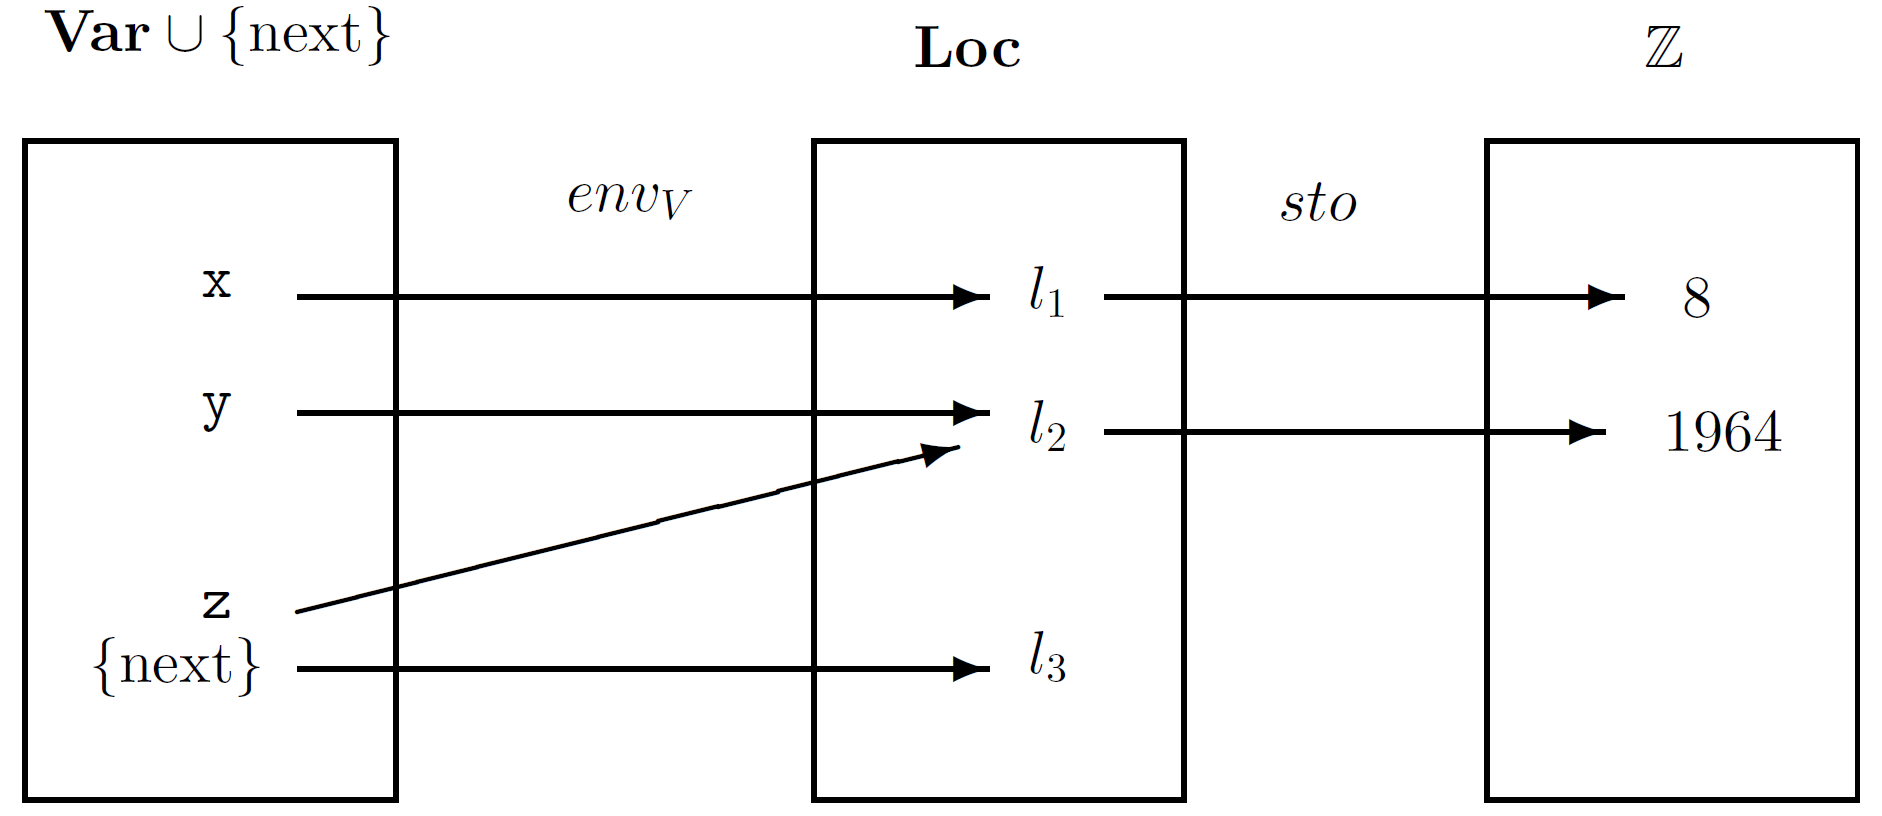
\includegraphics[width=0.8\textwidth]{figures/Environment_Store.png}
    \caption{Example diagram of the environment store model~\cite{Huttel2010}.}
    \label{fig:envstomodel}
\end{figure}


Arc has three environments: the variable environment, the function environment, and the task environment. To describe the semantics of these environments, some function, set and value names must be defined first. These definitions are presented in Table~\ref{tab:setsandfunctions}, and correspond to rules of Arc's \gls{cfg} described mathematically.

Following the standard of~\cite{Huttel2010}, sets are bolded and begins with a capital letter, while elements are not bolded.


\begin{table}[htb!]
    \centering
    \begin{tabular}{l}
        \toprule
        $\textbf{Val} = \textbf{Num} \cup \textbf{Bool} \cup \textbf{Char} \cup \textbf{Array} \cup \textbf{Pin}\ -$ Values                                                        \\
        $\textbf{Pin} = \textbf{PinValues} \times \textbf{Modes}\ -$ Pins are tuples of Arduino pins and modality                                                                  \\
        $\textbf{Array} = \mathbb{N} \rightharpoonup \textbf{Val} \setminus \textbf{Pin}\ -$ Arrays map numbers to non-pin values                                                  \\
        $\textbf{Par} = \textbf{Types} \times \textbf{Var}\ -$ Set of possible formal parameters                                                                                   \\
        $\textbf{Trig} = \{\epsilon, (\text{every} \times \mathbb{N}), (\text{when} \times \textbf{Expr}) \}\ -$ Set of triggers                                                   \\
        $v \in \textbf{Val}\ -$ Literal values                                                                                                                                     \\
        $x \in \textbf{Var}\ -$ Variable id                                                                                                                                        \\
        $f \in \textbf{Fun}\ -$ Function id                                                                                                                                        \\
        $t \in \textbf{Types}\ -$ Type names                                                                                                                                       \\
        $y \in \mathcal{P} (\textbf{Par})\ -$ Formal parameter lists                                                                                                               \\
        $r \in \mathcal{P} (\textbf{Var})\ -$ Reference parameter lists                                                                                                            \\
        $S \in \textbf{Stm}\ -$ Statements                                                                                                                                         \\
        $l \in \textbf{Loc}\ -$ An arbitrary location in \textbf{Loc}                                                                                                              \\
        next $\ -$ A special 'pointer' holding the value of the next element in \textbf{Loc}                                                                                       \\
        new $: \textbf{Loc} \rightarrow \textbf{Loc}\ -$ function to return succesor location                                                                                      \\
        \\
        $\textbf{Sto} = \textbf{Loc} \rightharpoonup \textbf{Val}\ -$ Set of stores                                                                                                \\
        $\textbf{Env}_V = \textbf{Var} \cup \{\text{next}\} \rightharpoonup \textbf{Loc}\ -$ Set of variable environments                                                          \\
        $\textbf{Env}_F = \textbf{Fun} \rightharpoonup \textbf{Stm} \times \mathcal{P} (\textbf{Par}) \times \textbf{Env}_V \times \textbf{Env}_F\ -$ Set of function environments \\
        $\textbf{Env}_T = \textbf{Stm} \times \mathcal{P} (\textbf{Var}) \times \textbf{Trig} \times \textbf{Env}_V \times \textbf{Env}_F\ -$ Set of task environments             \\
        \bottomrule
    \end{tabular}
    \caption{Sets and function definitions.}
    \label{tab:setsandfunctions}
\end{table}

\supervisor{Should we define types as $\{\epsilon, mut\} \times \textbf{Typenames} \cup \textbf{Typenames}$}


Additionally, we define the notation for updating a given environment $env_V \in \textbf{Env}_V$ we write $env_V[ x \mapsto l]$ to denote the update of $env_V$ given by


\begin{equation}
    env_V[x \mapsto l](y) =
    \begin{cases}
        env_V(y) & y \neq x \\
        l        & y = x
    \end{cases}
\end{equation}


\noindent and $env_F[ f \mapsto (S, y, env_V, env_F)]$ for $env_F$


\begin{equation}
    env_F[f \mapsto (S, y, env_V, env_F)](g) =
    \begin{cases}
        env_F(g)             & g \neq f \\
        (S, y, env_V, env_F) & g = f
    \end{cases}
\end{equation}


\noindent and similarly for a $sto \in \textbf{Sto}$ we write $sto[ l \mapsto v ]$ to indicate the update of $sto$ given by


\begin{equation}
    sto[l \mapsto v](l^\prime) =
    \begin{cases}
        sto(l) & l \neq l^\prime \\
        v      & l = l^\prime
    \end{cases}
\end{equation}
\todo{Missing $env_T$ definition. Should just be a set union an element.}

\noindent With the above definitions of the environment store model and the scope rules, Arc's declarations are described using operational semantics in Table~\ref{tab:arcscoperules}. Because of the static scope rules, the environments are contained within the results of the partial functions for variables and functions. Unlike the variable and function environments, the task environment is not a set of partial functions. This is because unlike function declarations, tasks are not used within other tasks, and as such does not need to map them.


\begin{table}[htb!]
    \small
    \centering
    \begin{tabular}{ll}
        \toprule
        $[PIN_{DECL}]$  & $\frac
            {\langle env^{\prime\prime}_V, sto[l \mapsto v] \rangle \rightarrow (env^\prime_V, sto^\prime)}
            {\langle \text{\#pin} \ x = (pv, mode), env_V, sto\rangle\rightarrow (env^\prime_V, sto^\prime)}$ \\ [12pt]
                        & where $(pv, mode) \in \textbf{Pin} $                                                \\
                        & and $(pv,mode) \rightarrow v $                                                      \\
                        & and $l = env_V(\text{next})$                                                        \\
                        & and $env^{\prime\prime}_V = env_V[x \mapsto l][\text{next} \mapsto \text{new}(l)] $ \\
        \\

        $[VAR_{DECL}]$  & $\frac
            {\langle env^{\prime\prime}_V, sto[l \mapsto v] \rangle \rightarrow (env^\prime_V, sto^\prime)}
            {\langle t \ x = expr, env_V, sto\rangle\rightarrow (env^\prime_V, sto^\prime)}$                  \\ [12pt]
                        & where $env_V, sto \vdash expr \rightarrow v $                                       \\
                        & and $l = env_V(\text{next})$                                                        \\
                        & and $env^{\prime\prime}_V = env_V[x \mapsto l][\text{next} \mapsto \text{new}(l)] $ \\
        \\

        $[FUNC_{DECL}]$ & $\frac
            {env_V \vdash \langle env_F[f \mapsto \langle S, y, env_V, env_F\rangle] \rangle \rightarrow env^\prime_F}
            {env_V \vdash \langle t \ f (y) \{S \}, env_F \rangle \rightarrow env^\prime_F}$                  \\ [12pt]

        $[TASK_{DECL}]$ & $\frac
            {env_{VF}\vdash \langle env_T[S, r, trig, env_V, envF] \rangle \rightarrow env^\prime_T}
            {env_{VF}\vdash \langle \text{task} \ (r) trig \{S\} \rangle \rightarrow env^\prime_T}$           \\
        \bottomrule
    \end{tabular}
    \caption{Arc's declarations and effects on scope defined with operational semantics.}
    \label{tab:arcscoperules}
\end{table}


To use the declared bindings we further define their calling and usage. Variables are immutable, and it therefore makes sense to have functions use call-by-value for the parameters. Function calls should not allow recursion, as this makes the runtime memory usage of the Arduino more stable.

Tasks are once again special. They are never called explicitly in Arc code, but the set of all declared tasks serve as the entrypoint of the program. This is done through parallel composition and invocation of all declared tasks, of which there must be at least one.

Also of importance is that the parameters of a task describe a mutable reference to a declared variable in $env_V$, that critically cannot be used in another task. This means that declarations are implicit calls with a call-by-reference model for its parameters.


\begin{table}[htb!]
    \centering
    \begin{tabular}{ll}
        \toprule
        $FUNC_{CALL}$ & $\frac{}{env_{VF} \vdash \langle f(e), sto\rangle \rightarrow sto^\prime}$ \\ [12pt]
                      & where $env_F(f) = \langle S, y, env^\prime_V, env^\prime_F \rangle$        \\
                      & and $\forall i | 0 \leq i \leq |y|$                                        \\
                      & and $e \in \textbf{Expr}^{ |y| }$                                          \\
                      & and $\forall i $                                                           \\

        $ENTRY$       & $\frac{}{}$                                                                \\ [12pt]
        \bottomrule
    \end{tabular}
    \caption{Semantics for function calls and task invocation.}
    \label{tab:callandentry}
\end{table}
\supervisor{How do I describe that each expression in the parameter list is evaluated and stored in a new location, with a variable $y_i$ from the formal parameter list pointing to that location?!}


\subsection{Type rules}\label{subsec:typerules}
Type rules are another set of contextual constraints. These rules make sure that code fragments do not mistreat types, for example in static typing, which Arc uses, it should not be possible to assign a number to a variable declared as a boolean~\cite{Sebesta2016}. The types that are valid in Arc are num, char, bool, and array, as descriped in~\ref{sec:inspiration}.

In the type checking semantics the types in the Arc language can be written as:
$T \in \{num, char, bool, N\} N \in \{ 0,\mathbb{N}\}$.
From now on semantics written mathmatticly will use T instead of type, if not given a specific type, in semantic type checking. If a specific type is needed, it is written instead of T.
N is not descriped ealier on what the types are in Arc, as it is not a type that can be declared. N is used for accessing an array, In C++ array access has to have a natural number, this is also implemented in Arc aswell. In C++ it is also 0-indexed~\cite{cppreferenceDataTypes}, which is withhold in Arc aswell.
In declarations and statements type checking, there will be an evaluation to $ok$ which means:

\blockcquote{Huttel2010}{The type of a declaration or a statement will simply be ok; we say that the declaration or statement is well-typed}

In Table~\ref*{tab:DeclTypeCheck}, the type checking for variables and functions are written. A specific type function declaration, has to type check if the return type is the same type as the declared function type. As task and a void function do not return, these declarations are always well-typed.


\begin{table}[htb!]
    \centering
    \begin{tabular}{ll}
        \toprule
        $[VAR_{DECL}] $  & $\frac{env \vdash expr : T}{env \vdash T \;x = expr : ok}$                            \\  [12pt]
        $[FUNC_{DECL}] $ & $\frac{env \vdash expr : T}{env \vdash T \;f() \{S; \;\text{return} \; expr\}  : ok}$ \\  [12pt]
        $[VOID_{DECL}] $ & $f()\{S\}  : ok$                                                                      \\
        \bottomrule
    \end{tabular}
    \caption{Arc type check for declarations.}
    \label{tab:DeclTypeCheck}
\end{table}


Now that the types has been clarified, it is important to look at operations a specific type can do.
The first type that will be clarified is num.
In Table~\ref{tab:num-rules} the expressions which the data type num only can do, is showed here.


\begin{table}[htb!]
    \centering
    \begin{tabular}{lll}
        \toprule
        $[ADD_{EXPR}] $                         & $\frac
            {env\vdash expr_1: num \quad env\vdash expr_2: num}
            {env\vdash expr_1 \;+\;expr_2: num}$
        \\ [12pt]
        $[SUB_{EXPR}] $                         & $\frac
            {env\vdash expr_1: num \quad env\vdash expr_2: num}
            {env\vdash expr_1 \;-\;expr_2: num}$
        \\ [12pt]
        $[MULT_{EXPR}] $                        & $\frac
            {env\vdash expr_1: num \quad env\vdash expr_2: num}
            {env\vdash expr_1 \;*\;expr_2: num}$
        \\ [12pt]
        $[DIVI_{EXPR}] $                        & $\frac
            {env\vdash expr_1: num \quad env\vdash expr_2: num}
        {env\vdash expr_1 \; / \; expr_2: num}$ & where $expr_2 \neq 0$
        \\ [12pt]
        $[REL_{EXPR}] $                         & $\frac
            {env\vdash expr_1: num \quad env\vdash expr_2: num}
            {env\vdash expr_1 \; OP \; expr_2: Bool}$                                 \\

                                                & where $OP \in \{<, >, \leq, \geq\}$

        \\
        \bottomrule
    \end{tabular}
    \caption{Type rules for num expressions in Arc.}
    \label{tab:num-rules}
\end{table}


The type num is the only type in Arc that can do arithmetic expressions, as it can only do arithmetic expressions on another num type, this can be seen in Table~\ref{tab:num-rules}. The end type of a arithmetic expression is still a num, as it makes changes to the value, not the type.

It is also the only type to check if a value is greater or smaller than an other num type when comparing. When doing a comparing of nums, the end type of the expression is a bool, as it true or false if the num is greater or less than the num it is compared to.


\begin{table}[htb!]
    \centering
    \begin{tabular}{ll}
        \toprule
        $[AND_{EXPR}] $ & $\frac
            {env\vdash expr_1: Bool \quad env\vdash expr_2: Bool}
            {env\vdash expr_1 \;\text{and} \;expr_2: Bool}$
        \\ [12pt]
        $[OR_{EXPR}] $  & $\frac
            {env\vdash expr_1: Bool \quad env\vdash expr_2: Bool}
            {env\vdash expr_1 \;\text{or} \;expr_2: Bool}$
        \\ [12pt]
        $[NOT_{EXPR}] $ & $\frac
            {env\vdash expr_1: Bool}
            {env\vdash \text{not} \; expr_1 : Bool}$
        \\
        \bottomrule
    \end{tabular}
    \caption{Type rules for bool expressions in Arc.}
    \label{tab:bool-rules}
\end{table}


The type bool has three expressions, that can be seen in Table~\ref{tab:bool-rules}. This means in the And, Or or Not expressions the expression getting type checked has to evaluate to a bool, the expressions will then evaluate to another type bool.


\begin{table}[htb!]
    \centering
    \begin{tabular}{ll}
        \toprule
        $[ARRAY_{EXPR}]$      & $ \frac
            {env\vdash expr_1: T \quad env \vdash expr_2 : N}
            {env\vdash expr_1[expr_2] : T}$
        \\ [12pt]
        $[PARENTHESIS{EXPR}]$ & $ \frac
            {env\vdash expr_1: T}
            {env\vdash (expr_1) : T}$
        \\ [12pt]
        $[EQUAL_{EXPR}] $     & $\frac
            {env\vdash expr_1: T \quad env\vdash expr_2: T}
            {env\vdash expr_1 \;== \;expr_2: Bool}$
        \\ [12pt]
        $[NOTEQUAL_{EXPR}] $  & $\frac
            {env\vdash expr_1: T \quad env\vdash expr_2: T}
            {env\vdash expr_1 \;!= \;expr_2: Bool}$
        \\
        \bottomrule
    \end{tabular}
    \caption{Type rules for other types of expressions in Arc.}
    \label{tab:expr-rules}
\end{table}


The type char does not have any expressions that only can be used on that type, therfore it only can use the expressions which bool and num can do as well. These type rules for expressions is written on Table~\ref{tab:expr-rules}. In the array expression the type N is used to describe the index for the array. The equal and not equal expression evaluate to a bool type, as it can only be true or false.


\begin{table}[htb!]
    \centering
    \begin{tabular}{ll}
        \toprule
        $[COMP_{STMT}] $     & $\frac
            {env \vdash stmt_1 :ok \quad env \vdash stmt_2 :ok}
            {env \vdash stmt_1\;;\;stmt_2: ok}$
        \\ [12pt]
        $[VAR-DECL_{STMT}] $ & $\frac
            {env \vdash expr : T}
            {env \vdash  T \;x = expr: ok}$
        \\ [12pt]
        $[ASSIGN_{STMT}]$    & $\frac
            {env\vdash x: T \quad env \vdash expr : T}
            {env\vdash x = expr: ok}$
        \\ [12pt]
        $[INDEX_{STMT}] $    & $\frac
            {env \vdash x : T \quad env \vdash expr : N \quad env \vdash expr : T}
            {env \vdash x[expr] = expr: ok}$
        \\ [12pt]
        $[BLOCK_{STMT}] $    & $\frac
            {env \vdash stmt :ok}
            {env \vdash \{stmt\}: ok}$
        \\ [12pt]
        $[CALL_{STMT}] $     & $\frac
            {env \vdash f:(x:T \rightarrow ok)\quad env \vdash expr:ok}
            {env \vdash call \;f(expr): ok}$
        \\ [12pt]
        $[RETURN_{STMT}] $   & $\frac
            {env \vdash expr: T}
            {env \vdash \text{return} \;expr: ok}$
        \\ [12pt]
        $[IF_{STMT}] $       & $\frac
            {env \vdash if (expr) : Bool \quad env \vdash stmt_1 :ok \quad env \vdash stmt_2 :ok}
            {env \vdash \text{if} (expr) \;stmt_1 \;\text{else} \;stmt_2: ok}$
        \\ [12pt]
        $[WHILE_{STMT}] $    & $\frac
            {env \vdash  expr : Bool \quad env \vdash stmt :ok}
            {env \vdash \text{while} (expr) \;stmt : ok}$
        \\ [12pt]
        $[FOR_{STMT}] $      & $\frac
            {env \vdash  y : T \quad env \vdash x : T \quad env \vdash block :ok}
            {env \vdash \text{for} (y \; \text{in} \; x) \; block : ok}$
        \\
        \bottomrule
    \end{tabular}
    \caption{Arc type check statements.}
    \label{tab:StatementTypeCheck}
\end{table}


The type checking for statements in Arc can be seen in Table~\ref{tab:StatementTypeCheck}. Type checking statements gives the same output as the declarations in "ok", as explained before means well-typed. A varable can be declared in a scope, therfore it has the same type check rules as in variable declaration, which can be seen in Table~\ref{tab:DeclTypeCheck}. Return uses an expression which evaluates to a type "T", this type is the same type as the type a function is declared with.

\chapter{Language semantics}\label{cha:languagesemantics}

Example semantics:

\begin{align*}
    [COMPOSITION] \quad &
    \frac
    {S_1, \sigma \rightarrow \sigma \prime \quad S_2, \sigma \prime \rightarrow \sigma \prime \prime}
    {S_1;S_2, \sigma \rightarrow \sigma \prime \prime}
    \\
    [RULE]     \quad    &
    \frac
    {Premises}
    {Conclusion}
\end{align*}

\begin{align*}
    [RULE]     \quad &
    \frac
    {Premises}
    {Conclusion}
    Side condition
\end{align*}

\chapter{Implementation}\label{cha:implementation}
This chapter covers the implementation of the Arc programming language. This includes a model of the compilation process and the compilation target, a short discussion of the visitor pattern, and a look at the implementation of the visitors, symboltable, typechecking, and scopechecking.


\section{Compiler}\label{sec:compiler}
The purpose of a compiler is to convert source code into target code. A generalized model of the compilation process can be seen in Figure~\ref{fig:generalcompilermodel}. In the case of the Arc compiler, the source code is text written in the Arc language.


\begin{figure}[htb!]
    \centering
    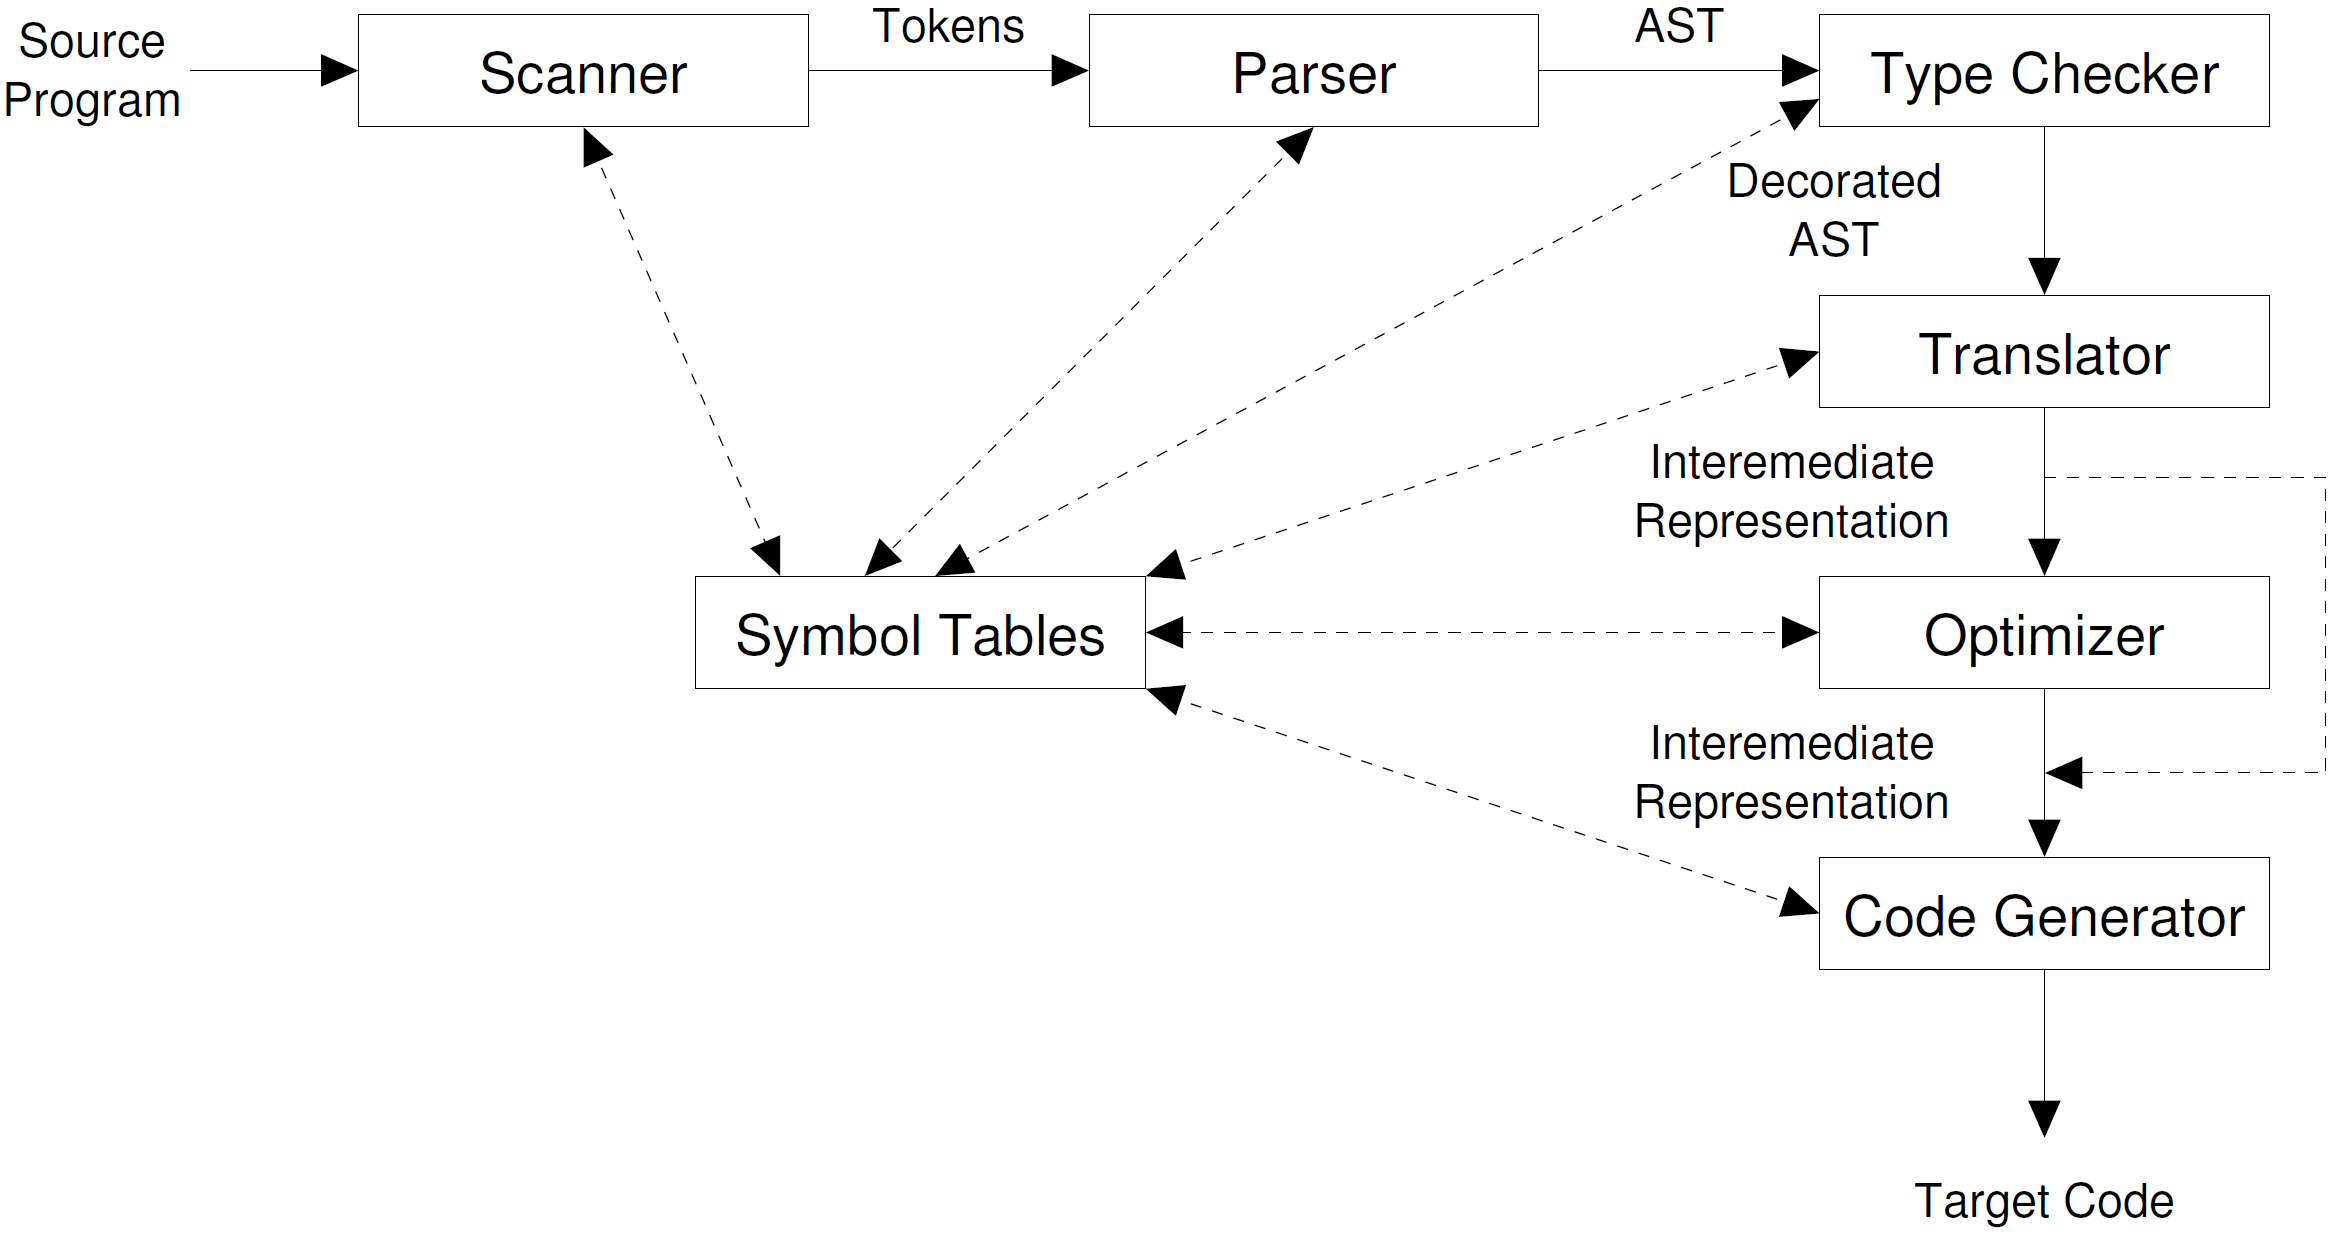
\includegraphics[width=0.8\textwidth]{figures/Full_Compiler.png}
    \caption{A textbook example of a compiler~\cite{CraftingCompiler}}
    \label{fig:generalcompilermodel}
\end{figure}


The target code is often low-level code for a particular system or runtime, but not always. When the target code is another high-level language, the process is also called transpilation. The Arc language is used for programming Arduinos, and so the compiler has to either generate Arduino-specific machine code or transpile it to the high-level Arduino language. Because the Arc language leverages the Protothreads library and its concurrency model for the Arduino, it makes sense for the Arc compiler to be a transpiler.

The Arc compiler follows many of the steps of the general model. Figure~\ref{fig:arccompilermodel} models the Arc compiler with some essential details.


\begin{figure}[htb!]
    \centering
    \begin{tikzpicture}[node distance=3cm]
        \begin{scope}[node distance=3cm,local bounding box=clusterA]
            \node (a) [state] {Scanner} node[below,scale=.7, xshift=60,yshift=-20]{Antlr};
            \node (b) [state, right of=a] {Parser};
            \draw[arrow, ->] (a) -- node[above,scale=.70,align=center]{Tokens} (b);
        \end{scope}
        \begin{scope}[node distance=3cm,local bounding box=clusterB]
            \node (c) [state, shift={($(b.east)+(2.3cm,0)$)}] {Type checker} ;
            \node (d) [state, shift={($(c.south)+(0,-1.5cm)$)}] {Scope checker};
        \end{scope}
        \node(clusterA_g)[cluster,fit=(clusterA)]{};
        \node(clusterB_g)[cluster,fit=(clusterB)]{};
        \node (q) [state, below of=clusterA_g] {Symbol table};
        \node (e) [state, shift={($(d.south)+(0,-1.5cm)$)}] {Code generator};
        \node (f) [shift={($(e.south)+(0,-1cm)$)}] {Target code};
        \node (start) [shift={($(clusterA.west)+(-2cm,0)$)}] {Source code};
        \draw[arrow, ->] (start) -- (clusterA_g);
        \draw[arrow, ->] (b) -- node[right,scale=.70,xshift=-16,yshift=7]{AST} (c) node[below,scale=.7, xshift=-30,yshift=-25, align=left]{Contextual\\ analysis};
        \draw[arrow, ->] (c) -- node[right,scale=.70,align=center]{AST} (d);
        \draw[arrow, ->] (d) -- node[right,scale=.70,align=center]{AST} (e);
        \draw[arrow, ->] (e) --  (f);
        \draw[arrow, dotted, <->] (q) --  (clusterB_g);

    \end{tikzpicture}
    \caption{The Arc compiler model.}
    \label{fig:arccompilermodel}
\end{figure}


Figure~\ref{fig:arccompilermodel} shows how the source code is first scanned into tokens and then parsed into an \gls{ast}. \gls{antlr} generates the lexer and parser for this from our grammar, hence the box around the scanner and parser. The \gls{ast} is then type-checked and scope-checked. The type and scope check rules are explained in more detail in section~\ref{sec:contextualconstraints}. Once the transpiler has done all of the necessary checks on the source code, it is ready to generate the Arduino code, which is also the final step of the compiler. The target code is now ready for the Arduino bases on the source code.
\section{Lexer and parser generation}

%what the lexer and parser is
%differences
%how it is used
%why it is used
%how we generate them
%alternatives
This section will briefly cover how the lexer and parser for Arc has been implemented, and what alternatives could have been used.

For Arc, \gls{antlr} has been used, for creating the grammer and also to generate both the lexer and parser. From writing the grammar, is was possible for \gls{antlr} to generate the lexer, parser and more.\cite{Parr2014} This made \gls{antlr} highly effective for designing Arc, as small changes to the grammar could easily be made, without having to re-create the lexer and parser everytime. Instead only the grammar had to be changed, and \gls{antlr} would generate a new lexer and parser, based on the new grammar.

The grammar was made in a file called 'arcv2.g4' which is an \gls{antlr} file, that \gls{antlr} recognizes and also the lexical rule were made in a file called 'lexerRules.g4'. With these files, \gls{antlr} could generate all needed files for the parser, the lexical analyzer, and other supporting files. These files can be seen in the image \ref{fig:lexerandparserfiles}

\begin{figure}[htb!]
    \begin{center}
        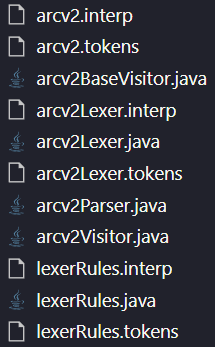
\includegraphics{figures/lexerAndParserFiles.png}
        \caption{Files generated for Arcs parser and lexical analyzer}
        \label{fig:lexerandparserfiles}
    \end{center}
\end{figure}

Figure \ref{fig:lexerandparserfiles} shows all files that \gls{antlr} generates, from the grammar rules and lexical rules. The file 'arcv2Parser.java' is the parser.\todo[]{Describe how the parser works and how it is used. Show code example!}


Another option to this could have been by writing out both the parser and lexer by hand, this could be very educational, as creating our own parser and lexer, would give in-depth knowledge of how they each work. But this would increase the time needed to create Arc considerably as, as mentioned previously, any minor change made in the grammar, would also mean going through the lexer and parser to fix them accordingly. This could lead to time wasted, which is a limiting factor for this project. Therefore it was decided to use the obviouse solution, to use the tools that readily avaliable. For this reason in particular, using \gls{antlr} to generate the lexer and parser for us, was the obviouse choice. 



\todo[inline]{Consinder adding examples of how we specifically have done it and discuss the files generated}

%The lexer, also called a lexical analyzer or scanner, takes a character stream and turns it into tokens. Tokens are a representation of something in a language, such as a num in Arc would be a token, that represents numbers. The lexer recognizes and can discard tokens of the character stream, so that the parser can ignore them. This includes tokens such as comments and whitespaces, that the parser does not need to concern itself with. If the lexer did not discard these tokens, that parser would constantly have to check for them. These tokens are then passed to the parser, that makes syntatic sense of them. It compares the tokens and their structure to the grammar of the specific language.\cite{Parr2014}



\section{Visitor pattern}\label{sec:visitorpattern}\feedback{We still working on this section, and unsure what }
This section will briefly discuss what the visitor pattern is, how it is used in Arc, and why it is used. ANTLR provides two methods of traversing a \gls{cst}, listeners and visitors. 

The listener pattern, is not responsible for calling methods to traverse the tree. ANTLR generates enter and exit methods for each rule, these methods are then called when the walker encounters a node. The benefits of using the listener pattern, is that it is automatic, and the methods created do not have to explicitly visit all their child nodes\cite{Parr2014}. \feedback{We are unsure of how correct this actually is, taken from: Page 18}

The visitor pattern, is a method used to traverse the \gls{cst} in a specific manner, where methods are used to visit each child node. By using the visitor pattern, there is more control of how the traversal of the \gls{cst} is done, and how much of the \gls{cst} is visited. ANTLR can generate a visitor interface, this interface is created from Arcs grammar, and creates all the needed visitor methods. These act as boilerplate for Arcs needed visitor methods, that can then be written out to do excatly as needed\cite{Parr2014}. 

For Arc there is made use of the visitor pattern, because it is not neccecary, for Arc, to visit all nodes, since for some of them it is know what will follow. It is also the more secure option, as it gives the option to be more specific about what happens for each node. This is especially good for futureproofing, as there might be certain things that had not been prdicted, and can therefore be specifically fixed.


%Options
%pros and cons of both
%How is it used
%How do we use it


%Vi vil ikke altid ind i alle noder, fordi det ikke er nødvændigt
%Det er sikre valg, da vi kan være specifikke for hver node, hvis der er noget vi ikke har forudset
%Future proof

\section{Scoping}\label{sec:scoping}
Scoping describes where variables are visible, meaning when a variable can be referenced or assigned. This is an important part of a programming language, since identifiers often are reused, such as i for an iteration. Because of this, scoping is used to differ variables from eachother and also to either allow references to variables or to inhibit reference. For this there are two general types of scoping, dynamic and static.

Static scoping, means that the scope of variabels is determined staticly, meaning it is done before execution of the program. Static scope is used in many languages, including C and C\#. Static scoping is said to be more readable, since the code often shows directly the value of the variable. When a reference to a variable is found, following previous references and finally the assignment to that variable, the value of that variable can be determined. An example of static typing, can be seen in Listing~\ref{lst:scopeexample}.

Dynamic scoping, means that the scope of variabels is determined during run time of the program. Dynamic scope is used in languages including Perl and Common Lips. Dynamic scoping works by using the calling sequence of subprograms to determine the value of eks. a varible. Because of this it cannot be determined staticly as static scoping, and mus tbe done during run time. Dynamic scoping decreases readability of the code, since it can be difficult to know the exact calling sequence of subprograms that contain references to a variable~\cite{Sebesta2016}. An example of how dynamic scoping works, can be seen in Listing~\ref{lst:scopeexample}.\todo{Seems more relevant to the section on language design instead. This section should be about the concrete implementation of Arcs scoping rules than the general ideas of scoping.}

\begin{listing}[htb!]
    \begin{minted}{C}
        int a = 5;

        int fun1(x){
            return x + a
        }
        int fun2(){
            a = 10;
            return fun1(10);
        }
        print(fun2());
    \end{minted}
    \caption{An example of how static and dynamic scope differs}
    \label{lst:scopeexample}
\end{listing}

When using static scoping, Listing~\ref{lst:scopeexample} will print '15', because of the variable a assigned in the beginning being a global variable, and fun1 using that with the x given as it's parameter. Compared to dynamic scoping where there would be printed '20', this is because of the previously mentioned calling sequence. The variable 'a' is assigned to '5', but then in fun2() it is updated to '10' and this value is then used in fun1().

Arc uses static scoping, as it more simple to read and understand for users, and C++ uses a variant of static scoping. Because of this it makes sense for Arc to also a simillar scoping.

In the implementation the creation of the different scopes is primarily archieved through Block structure we use in our syntax. The visitation of this structure is when we push and pop the stack of scopes. This can be seen in Listing~\ref{lst:VisitBlock} Where the visitor visit this node we first push to the context then visit its children and Afterwards we pop this scope that is no longer needed.

\begin{listing}[htb!]
    \begin{minted}{java}
    public AST_node visitBlock(arcv2Parser.BlockContext ctx) {
        symbolTable.push();
        AST_node block = new Variable_declaration_node("block");
        List<arcv2Parser.StatementContext> list = ctx.statement();

        for (arcv2Parser.StatementContext statementContext : list) {
        visit(statementContext);   
        }
        symbolTable.pop();

        return block;
    }
    \end{minted}
    \caption{VisitBlock from our evalvisitor}
    \label{lst:VisitBlock}
\end{listing}

Our Scoping rules are implemented everywhere in our semantic visitor, an example of how it works can be seen in Listing~\ref{lst:ScopeImplementationExample} where it can be seen that our forloop use a call to our symbolTable to check if the identifier given as input has been declared. This archieved using the get function showed earlier, which returns null if it does not exist.

\begin{listing}[htb!]
    \begin{minted}{java}
    @Override public AST_node visitForloop_statement(arcv2Parser.Forloop_statementContext ctx) { 
        ...
        SymbolHashTableEntry entry = symbolTable.get(ctx.IDENTIFIER(1).getText());
        if (entry == null) {
            throw new RuntimeErrorException(null, "this identifier '" + ctx.IDENTIFIER(1).getText() + "' does not exist" );
        }
        ...
    }
    \end{minted}
    \caption{The SymbolHashTableEntry class}
    \label{lst:ScopeImplementationExample}
\end{listing}



%What is scoping
%Blocks
%Types of scoping
%Pros and cons of the two
%What does Arc use
\section{Type checker}
This section will discuss the type checker for Arc, how it is structured and also show examples of how it works.

The type checker verifies that operands of an operator are of compatible types, and if not, throws an error, with an error message for the user to use to fix the issue \cite{Sebesta2016}. It does this by walking through the \gls{cst} from the bottom-up, with a visitor pattern \cite{Parr2014}. An example of the type checker throwing an error would be the case where a user tries to use the plus operand on a num and a char, this will throw an error to the user telling them, that this operation is not valid in Arc.

There are two ways to type check, static and dynamic type checking. Static type checking works on compile time, dynamic type checking is done during run time. Usually it is better to use static type checking, as it catches errors earlier compared to dynamic type checking, and is less costly \cite{Sebesta2016}. Altough dynamic typing allows for more flexablility when writing code, as in languages such as Python where types are not needed to be declared, but simply values are to be given.

In Arc there will be made use of a static type checker, this is because the language that Arc transpiles to is C++ which is a staticly typed language. For this reason it makes sense for Arc to also be a staticly typed language, so it can be easily used with the Arduino, which uses a language that is a subset of the C++ language. \todo{indsæt evt ref til at Arduino bruger C++} Combined with the previously mentioned benefits of using a staticly typed language, it seemed like the obviouse decision to have Arc be a staticly typed language. Although an argument could be made that Arc should be made a dynamicly typed language, since often dynamicly typed languages, such as Python, tend to be faster to write code in. Since time is a limiting factor for our definition of a hobbyist, it would make sense to make a language that encourages less time spent writing code. But since Arc is only made to work with simple concurrency, this time spent on writing code, might not give as much of a gain, as in a standard language. \todo{This just sounds like bullshit -gustav "true"}

\begin{listing}[htb!]
    \begin{minted}{java}
        SymbolHashTableEntry entry = symbolTable.get(ctx.IDENTIFIER().getText());
        

        //TODO  this needs to handle arrays (should we even allow array assignment)
        AST_node expression = visit(ctx.expression(0));

        if (entry == null) {
            throw new RuntimeException(" this varible '" + ctx.IDENTIFIER().getText() + "' does not exist");
        }
        else if (entry.Mutability != true) {
            throw new RuntimeException(" this varible '" + ctx.IDENTIFIER().getText() + "' is not mutable and therefore cannot be assigned to");
        }
        else if (entry.Type !=  expression.type) {
            throw new Expression_type_exception("the assingment expression has bad typing");
        }
        else{
            symbolTable.insert(entry);
        }
    \end{minted}
    \caption{Code snippet of Arcs type checker}
    \label{lst:typecheckerexample}
\end{listing}
\todo[inline]{Feel like it is missing a function name}
\todo{this is actually a bad example as it shows too much you talk about alot of checks that arent type check like scope cheks}
\ref{lst:typecheckerexample} shows am example of Arcs typechecker. This example shows the part of the typechecker, handles assignments. It does this by creating 'entry' of the class SymbolHashTableEntry and assigns it to the contents of a ctx file\tode{yeah, naw. thats not whats happening were creating an entry and assigning to it the result of a lookup in the symbolTable based on the IDENTIFIER that were assigning to.}. Then it creates 'expression' of the AST\_node class, and uses a visitor method to assign it to the first expression of the \gls{cst}\tode{this is closer. here were creating a ast nodes and assingning it the result of a visit to a expression. and in our visitor a visit always returns a ast node}. It is then evaluated in a sequence of if statements, to ensure that the assignment is a legal action in Arc. First checking if the entry even exists, then if the entry is mutable and finally checking if the types of the entry and expression are equvilant. If the entry passes all the checks, it is then inserted into the sybol table. If it does not pass one of the checks, an exeption is thrown and a relevant error message is given.
\todo[inline]{Entire paragraph has to be checked to ensure it is correct}


%dynamic vs static typechecking
%formal definitions som cagala?
%Why is it important to have a typechecker
%argument could be made that a dynamic typed language would be better for hobbyists since time is a limiting factor for them, and in general dynamicly typed languages are faster to write code in.
\section{Code Generation}\label{sec:codegeneration}
This section will explain the code gen part of the compiler. In this part of the implementation, the target
code is generated. The target code is the Arduino language, which is essentially c/c++ with some Arduino constructs. The code is generated using another visitor pattern similar to the one we use for semantic analysis. It follows the divide and conquer principle and uses the antlr generated \gls{ast}. It then generates the code going through the \gls{ast} and passing the generated code between the nodes using our CodeGenStringObject.

\begin{listing}[htb!]
    \begin{minted}[label=CodeGenStringObject class definition]{java}
    public class CodeGenStringObject {
    public String GlobalScope = "";
    public String Setup = "";
    public String Loop = "";
    public String Type_Coverter (String input){
        if(input.equals("mut num") || input.equals("num" )){
            input = "float";
        }
        if(input.equals("mut char")){
            input = "char";
        }
        if(input.equals("mut bool")){
            input = "bool";
        }
        return input;
        }
    }
    \end{minted}
    \caption{CodeGen object used in code generation.}
    \label{lst:code gen object}
\end{listing}

We use the CodeGenStringObject because a node sometimes will generate code in 3 different places of the final code at once. Hence we have made an object containing three different strings and a method. The three strings each correspond to one of the three areas that can be generated to the three sections, GlobalScope, the Setup structure, and the loop structure. This makes it possible to do all code-gen simply in a single visit of the three because it's unnecessary to keep track of 3 different placements in the file and switch between writing in them. The final code gen is done by using the final CodeGenStringObject and simply inserting the three strings into the file in order. \todo{this needs to be more clear, and use an example to show it} The method in CodeGenStringObject is simply used in code-gen to rewrite the types that we have in the input to the corresponding types in c++.

The visitor pattern is very similar to the one used for type checking, scope checking, etc. This is because they are all extensions of the arcv2basevisitor. This is possible because they're using the same Antlr generated \gls{ast} as input. A custom \gls{ast} is not created because it would look very similar to the one Antlr would generate because our grammar generally creates a quite shallow tree, so the \gls{ast} would not be very different in structure. It would also make it necessary to do a lot of reimplementing a lot of methods and data structures that antlr \gls{ast} has baked in. Therefore we keep using the antlr \gls{ast} since there isn't a lot of upside to making a new one. \todo{does this sound convincing?}


In figure \ref{lst:codegenexpression} we see a simple example of how The code gen visitor works. Here we see it first creates two objects of the class CodeGenStringObject shown earlier. One is named cpp, which stands for c + +, and one is named temp since it is temporary and does not get returned out of the method. Then we assign temp the result, and the global scope of this object is then added to cpp. Only the global scope is added since we know only different expressions can exist within an expression, and none of our expressions add to anything other than the global scope. Then we use the result of ctx.plus to check if we should add a plus or minus to cpp. Ctx.plus equals either a plus terminal or null if it doesn't exist; hence this is possible. In the end, we do the same thing again with the visit, just with the second expression, which is then added to cpp, and cpp is returned to the parent of this node. We don't check if more exist because only two can exist in a plus-minus ctx. So basically, this visitor visits a node, adds the result of visiting its children to it, and then returns it to its own parent, which is how our code-gen works.


\begin{listing}[htb!]
    \begin{minted}[label=CodegenVisitor.visitPlusMinusExpression]{java}
    public CodeGenStringObject visitPlus_minus_expression(arcv2Parser.Plus_minus_expressionContext ctx) {
        CodeGenStringObject cpp = new CodeGenStringObject();
        CodeGenStringObject temp = new CodeGenStringObject();
        temp = visit(ctx.expression(0));
        cpp.GlobalScope += temp.GlobalScope + " ";

        if (ctx.PLUS() != null) {
            cpp.GlobalScope += "+ ";
        } else {
            cpp.GlobalScope += "- ";
        }
        temp = visit(ctx.expression(1));
        cpp.GlobalScope += temp.GlobalScope;

        return cpp;
    }
    \end{minted}
    \caption{code gen object used in code gen}
    \label{lst:codegenexpression}
\end{listing}


A different interesting part of the code-gen visitor is the task declaration visit which is visible here\ref{lst:codeGenTask}.
This one has a bit more happening. The first part until line??? describes the creation of the cpp CodeGenStringObject and all the things that should be added to the global scope every time a task is declared. It also creates a name for the thread, which will be used in c++. This is necessary because the tasks in arc do not have names. These names are generated generically based on a counter function which can be seen at the button, so they end up being named pt0thread, pt1thread, etc.
That means all the things need to be inserted to create a protothread. Afterward, we see three control structures, an if, else if, and an else, which describe the three different ways we describe a task.

Firstly in line??, we have an if statement that, similarly to the previous example, checks if there is an every and if there is, we enter the if statement. Inside First that happens is the creation of a list of all the statements that are the immediate children of task declaration. This list is then iterated through, and the result of the visits to the individual children are added to the cpp in order. This Finishes with adding what is essentially a call to a protothreads function sleep that sleeps the thread for the amount of time specified in the Number, which corresponds only to every because it only exists if there is an every.

Second is the case where we use a when. In that case, we add an if statement inside of the protothread and insert the product of a visit to the boolean expression that we know has to exist if there is a when per our grammar. On line??, we again see the construct used to add the statements.

The Third else case is just the same statement iteration without anything extra.


how it works with example -tasks
\begin{listing}[htb!]
    \begin{minted}[label=CodegenVisitor.visitTaskDeclaration]{java}
    @Override
    public CodeGenStringObject visitTask_declaration(arcv2Parser.Task_declarationContext ctx)
    {
        CodeGenStringObject cpp = new CodeGenStringObject();
        String ptName = "pt" + Integer.toString(get_task_number());
        String ptNameThread = ptName + "thread";

        cpp.GlobalScope += "pt " + ptName;
        cpp.GlobalScope += ";\n";
        cpp.GlobalScope += "int " + ptNameThread + "(struct pt *pt) { \n PT_BEGIN(pt);\n for(;;){ \n";

        if (ctx.EVERY() != null) {
            List<StatementContext> list = ctx.statement();
            for (StatementContext statement : list) {
                cpp.GlobalScope += visit(statement).GlobalScope;
            }
            cpp.GlobalScope += "\nPT_SLEEP(pt, " + ctx.NUMBER().getText() + ");\n";
            cpp.GlobalScope += "\n}\n";
        } else if (ctx.WHEN() != null) {
            cpp.GlobalScope += "if (" + visit(ctx.expression()).GlobalScope + ") { \n";
            List<StatementContext> list = ctx.statement();

            for (StatementContext statement : list) {
                cpp.GlobalScope += visit(statement).GlobalScope;
            }
            cpp.GlobalScope += "\n}\n";
        } else {
            List<StatementContext> list = ctx.statement();
            
            for (StatementContext statement : list) {
                cpp.GlobalScope += visit(statement).GlobalScope;
            }
            cpp.GlobalScope += "\n}\n";
        }
        cpp.GlobalScope += "PT_END(pt);\n}";
        cpp.Setup += "PT_INIT(&" + ptName + ");";
        cpp.Loop += "PT_SCHEDULE(" + ptNameThread + "(&" + ptName + "));";

        return cpp;
    }
    \end{minted}
    \caption{Code generation of task declarations.}
    \label{lst:codeGenTask}
\end{listing}

\begin{listing}
    \begin{minted}[label=CodegenVisitor.getTaskNumber]{java}
        private int count = 0;
        public int get_task_number() {
            int temp = count;
            count += 1;
            return temp;
        }
    \end{minted}
    \caption{Keeping track of the number of tasks.}
    \label{lst:codeGenTaskNumber}
\end{listing}





\section{MOVE ME EVENTUALLY}
This section contains text that has to be moved to proper sections.

\subsection*{Arc implemementation of the sample project}
The sample project implemented in Arc.

\begin{listing}[htb!]
    \begin{minted}[label=Arc example]{text}
        #pin BUTTON_PIN(12, OUTPUT);
        mut num buttonState = 0;
        mut bool ledState = HIGH;

        task(bool ledState) every 1000 {
            ledState = not ledState;
            digitalWrite(LED_BUILTIN, ledState)
        }

        task(num buttonState) {
            buttonState = digitalRead(BUTTON_PIN);
            Serial.Println(buttonState);
        }
    \end{minted}
    \caption{Project example implemented in Arc, assuming print is possible.}
    \label{lst:arcexample}
\end{listing}

\chapter{discussion}\label{cha:discussion}

This chapter will cover the discussion of how well Arc has lived up to its language criteria, and how well the project lives up to the learning goals for the semester.

\section{Language design}

This section will discuss the language design of Arc, the descisions made and what could have been done differently.

\subsection{Design descision} 

As mentioned in section \todo{Add section reference}, Arc makes use of a single data type to represent all numbers, called num and is treated as a float. Compared to many other languages that include multiple different type to represent different categories of numbers. This descision was made, based on the idea that using a single data type that represents all numbers, would be easier and faster to work with, compared to a system that would use e.g. Int and Float. \todo{Operationalsemantics mentions moving a section here, that further discusses num vs int and float}

Another design descision worth discussing is the choice of scope and type rules of Arc. \todo[inline]{Read section 3.4 and continue from here}
%num vs int + float
    %num is easier to understand
        %Can lead to arithmetic issues
%Do tasks work as a construct
%Scope rules, type rules
    %Call by value vs call by reference
    %Semantics

\subsection{Resemblence to C}
%The good
Arc uses a simillar syntax to that of C, this was done intentionally, but an argument can be made wether that was a good descision or not. C is a popular language and has a syntax simillar to that of many other languages. Therefore with Arc having a syntax that resembles C, would imply that users learning how to program with Arc, would have an easier time in the future learning new programming languages. Also if a user has had just a little experience with another programming language, that also has a simillar syntax to C, Arc would be more recognizable for them, and they should be able to learn how to work with concurrency faster. Arduino uses a subset of C++, and since C++ and C use very simillar syntax, it was easy to translate much of Arcs syntax to something that was able to compile on the Arduino.
%The bad
Although it could be argued that using a syntax that resembles C, has limited the creativity of creating a unique programming language, that is specified to work with concurrency. It can be seen in the syntax of Arc, that does not work with concurrency, that much has not been changed compared to that of C, apart from the for loop, that resembles that of Python. An issues with this could be seen in a case where a user has difficulties understanding and using regular C.\question{Maybe just remove this sentence} This is often how new languages are made, taking inspiration from many other languages and implementing them into their own. The reason for this, is because the syntax for C is widely used, and there is no reason to try and make changes that do not serve any particular purpose. \question{Måske skrive: and there is no reason to try and make changes for the sake of making changes}

%Challenges with concurrency
    %Complex subject
    %Simplified and limited use of concurrency
    %Arduino does not support true concurrency
    %Better start to paragraph
The design for Arc is made in a way, to give hobbyists a simple way to work with and learn how to use concurrency with an Arduino, to do this the library Protothreads has been used. Some challanges that were found during production of Arc, included that concurrency is a complex topic and proved hard to understand and use at times. Therefore it was difficult to simplify it to a level, that was assumed to be understandable for hobbyists. Arc ended up with three main concurrency structures, \textbf{When}, \textbf{Where}, and the idle task. These task were made in an effort to simplify concurrency to resemble somewhat spoken language. Because of this, there was given limited control over the concurrency structures, other libraries that were researched included options such as being able to give priorities to certain tasks. This was done in an effort to reduce complexity of the tasks as much as possible, since it was assumed that hobbyists who needed more complex functionality, would find and use other libraries. But an argument could be made, that the structures have been simplified too much and abstracted away options that could be useful for users. More options could have been made avaliable for users to work with, for better control over the concurrent tasks running. This might have slightly increased the complexity of Arc, but could also lead to better use of the concurrent tasks. For this project, the simplicity of Arc was a priority, therefore the more simplified concurrent tasks were used. \question{Needs to draw more attention to the aspect of resembling C}

\question{Show how Arc differs from Protothreads and discuss if it makes sence to use Arc over it}




%--------------------NOTES-------------------------
%Learning goals for semester - Show we have understood them or misunderstood them
%   Have we actually used visitor pattern, if not why?
%Did we live up to our language criteria
%Problem statements
%Arduino
%Should our compiler contain more phases
%Should we have included a front end for our compiler - flags
%Was ANTLR a good tool for us
%   Antlr good for us since we are inexperinced and had to make many changes
%Things we did nnot include in Arc (print and read) - Should we have included it
%   Our example of concurreny languages uses Serial(print) but Arc does not have that.

%What did we do
%Did we live up to our goals and the goals set for us
%What did we not live up to
%   Usability test/general testing - Do we have enough
%   Time constraints or lack of experience
%What could or should we have done differently
%What would we like to improve in the future
%*Do we want to mention tools we used? Github, Discord, Notion, and Teams
%Inlude a code snippet of Protothreads and how it would look in Arc to show difference
    %discuss how Arc differs from Protothreads


%-----------------------SETUP---------------------------
%Introduction to discussion section
%Language Design
    %Did we live up to our language criteria
        %Go through all characteristics and determine if Arc follows the priorities made
    %Inlude a code snippet of Protothreads and how it would look in Arc to show difference
        %discuss how Arc differs from Protothreads
    %Arduino
    %Learning goals for semester - Show we have understood them or misunderstood them
    %Problem statement
    %Should our compiler contain more phases
    %Things we did not include in Arc (print and read) - Should we have included it
        %Our example of concurreny languages uses Serial(print) but Arc does not have that.
%Implementation
    %Was ANTLR a good tool for us
        %Antlr good for us since we are inexperinced and had to make many changes
    %Have we actually used visitor pattern, if not why?
    %Should we have included a front end for our compiler - flags
%Test
    %Usability test/general testing - Do we have enough
    %How would we have improved on testing and why did we not
%Future works
    %What would we like to improve in the future


\printglossaries

\printbibliography[heading=bibintoc]
\label{bib:mybiblio}

\appendix
\chapter{Reading instructions}
These are the reading instructions for the next supervisor meeting. 

\section{Review priority}
\begin{enumerate}
    \item Read and answer all green notes
    \item Read all of chapter \ref{cha:introduction}
    \item Read sections \ref{sec:arduino} and \ref{sec:concurrency}
    \item Read sections \ref{sec:inspiration}, \ref{sec:syntax specification}, and \ref{sec:concurrency structures}
    \item Ignore sources that are not input properly yet, except if they are marked by a green note. 
\end{enumerate}

\end{document}